\documentclass[aspectratio=169,mathserif]{beamer}
\usepackage{pgfpages}
\usepackage{dsfont}
\usepackage{tikz}
\usetikzlibrary{calc}
\usetikzlibrary{graphs}
\usetikzlibrary{cd}
\usetikzlibrary{patterns}
\usetikzlibrary{backgrounds}
\usetikzlibrary{shapes}
\usetikzlibrary{decorations.pathmorphing}
\usetikzlibrary{decorations.pathreplacing}
%\usepackage{bussproofs}
\usepackage{stmaryrd}
%\usepackage{colortbl}
%\usepackage{booktabs}

% ACM palette {{{
\definecolor[named]{ACMBlue}{cmyk}{1,0.1,0,0.1}
\definecolor[named]{ACMYellow}{cmyk}{0,0.16,1,0}
\definecolor[named]{ACMOrange}{cmyk}{0,0.42,1,0.01}
\definecolor[named]{ACMRed}{cmyk}{0,0.90,0.86,0}
\definecolor[named]{ACMLightBlue}{cmyk}{0.49,0.01,0,0}
\definecolor[named]{ACMGreen}{cmyk}{0.20,0,1,0.19}
\definecolor[named]{ACMPurple}{cmyk}{0.55,1,0,0.15}
\definecolor[named]{ACMDarkBlue}{cmyk}{1,0.58,0,0.21}
%}}}

% Parameters {{{
\newcommand{\figsize}{\small}
\usecolortheme[named=ACMDarkBlue]{structure}
%\setbeameroption{show notes on second screen}

\addtobeamertemplate{navigation symbols}{}{%
    \usebeamerfont{footline}%
    \usebeamercolor[fg]{footline}%
    \hspace{1em}%
    \insertframenumber/\inserttotalframenumber
}

\AtBeginSection[] % Do nothing for \section*
{
%\begin{frame}<beamer>
%\frametitle{Outline}
%\tableofcontents[currentsection]
%\end{frame}
\frame{\sectionpage}
}
%}}}

% Macros {{{

% Some of the macros I defined trip up latexdiff,
% so I separate them in this file.
% vim: foldmethod=marker

% Notations
\newcommand{\kw}[1]{\ensuremath{ \mathsf{#1} }}
\newcommand{\ifr}[1]{\mathrel{[{#1}]}}
\newcommand{\que}{\circ}
\newcommand{\ans}{\bullet}
\newcommand{\vref}{\le_\kw{v}}
\newcommand{\mext}{\le_\kw{m}}
\newcommand{\refby}{\preceq}
\newcommand{\scref}{\sqsupseteq}
\newcommand{\screfd}{\sqsubseteq}
\newcommand{\unitset}{\mathds{1}}

% Multi-letter language interfaces
\newcommand{\li}[1]{\mathit{#1}}
% Calling conventions (language interface boundaries)
\newcommand{\cc}[2]{{ \kw{#1#2} }}

% Pointers for justified sequences %{{{

% Parameters
\newcommand{\pshift}{1.6ex}
\newcommand{\pcdist}{1}
\newcommand{\pcangle}{60}

% Pointer hook
\newcommand{\ph}[1]{%
  \tikz[remember picture]{\coordinate (#1);}}

% Pointer to
\newcommand{\ptc}[2]{%
  \tikz[remember picture,baseline,>={Latex[round,length=3.6pt]}]{
    \draw[->,#2]
      let \p{dest} = (#1),
          \n1 = {pow(veclen(\x{dest}, \y{dest}), 0.5) * 1.5},
          \p1 = ($(0,0)+(0,\pshift)$),
          \p4 = ($(\x{dest},0)+(0,\pshift)$),
          \p2 = ($(\p1)!\n1*\pcdist!-\pcangle:(\p4)$),
          \p3 = ($(\p4)!\n1*\pcdist!+\pcangle:(\p1)$) in
        (\p1) .. controls (\p2) and (\p3) .. node[pos=0.5] (top) {} (\p4);
    \pgfresetboundingbox
    \path[use as bounding box] (0,0 |- top);
}}
\newcommand{\pt}[1]{%
  \ptc{#1}{gray}}
\newcommand{\bpt}[1]{%
  \ptc{#1}{black,thick,>={Latex[round,length=4pt]}}}

% TikZ setup
\pgfdeclarelayer{tint}
\pgfdeclarelayer{nodes}
\pgfsetlayers{tint,background,main,nodes}
\selectcolormodel{cmyk}

% Parameters for diagrams
\newcommand{\stens}{0.6}

% The intensity of colors in figures and row highlighting respectively.
% These should be the same, otherwise they are just confusing to look at
% side by side, especially on a printout.
\newcommand{\filltint}{!35}
\newcommand{\tbltint}{\filltint}

% Colors used in the World transitions section
\newcommand{\colorA}{ACMDarkBlue}
\newcommand{\colorB}{ACMDarkBlue}
\newcommand{\internalA}[1]{\textcolor{\colorA}{#1}}
\newcommand{\internalB}[1]{\textcolor{\colorB}{#1}}

% Refinement tiles {{{

\newenvironment{tile}[1]{%
  \begin{tikzpicture}[baseline,yscale=0.36,xscale=0.5]
    \figsize
    \tikzset{to path={
      .. controls ($(\tikztostart)!\stens!(\tikztostart -| \tikztotarget)$)
              and ($(\tikztotarget)!\stens!(\tikztotarget -| \tikztostart)$) ..
      (\tikztotarget) \tikztonodes}}
    \tikzset{#1}
    % Coordinates for things on the left
    \coordinate (TL) at (-1,1);
    \coordinate (L) at (-1,0);
    \coordinate (BL) at (-1,-1);
    \coordinate (TLB) at (-0.3,1);
    \coordinate (BLB) at (-0.3,-1);
    % Coordinates for things on the right
    \coordinate (TR) at (1,1);
    \coordinate (R) at (1,0);
    \coordinate (BR) at (1,-1);
    \coordinate (TRB) at (0.3,1);
    \coordinate (BRB) at (0.3,-1);
    % Center node, for crossing
    \coordinate (T) at (0,+1.5);
    \node[circle,inner sep=2pt] (C) at (0,0) {};
    \coordinate (B) at (0,-1.5);
    % Computed coordinates
    \coordinate (TLC) at ($(T-|L)$);
    \coordinate (BLC) at ($(B-|L)$);
    \coordinate (TRC) at ($(T-|R)$);
    \coordinate (BRC) at ($(B-|R)$);
}{%
  \end{tikzpicture}%
}
\newcommand{\simproof}[2]{%
  \begin{pgfonlayer}{nodes}
    \node[draw,rectangle,fill=white,rounded corners=2pt,minimum height=0.5cm,minimum width=0.8cm] at #1 {#2};
  \end{pgfonlayer}
}
\newcommand{\drawsc}{%
  \draw[thick,rounded corners=1mm]
}
\newcommand{\fillleft}[1]{%
  \begin{pgfonlayer}{tint}
    \fill[#1] (TLC) rectangle (B);
  \end{pgfonlayer}
}
\newcommand{\fillright}[1]{%
  \begin{pgfonlayer}{tint}
    \fill[#1] (T) rectangle (BRC);
  \end{pgfonlayer}
}
\newcommand{\filltop}[1]{%
  \begin{pgfonlayer}{tint}
    \fill[#1] (TLC) rectangle (R);
  \end{pgfonlayer}
}
\newcommand{\fillbot}[1]{%
  \begin{pgfonlayer}{tint}
    \fill[#1] (L) rectangle (BRC);
  \end{pgfonlayer}
}
\newcommand{\fillboth}[1]}}



% adjust borders on this
\renewcommand{\simproof}[2]{%
  \begin{pgfonlayer}{nodes}
    \node[draw,rectangle,fill=white,rounded corners=2pt,
      minimum height=0.5cm,minimum width=0.8cm,inner sep=2pt] at #1 {#2};
  \end{pgfonlayer}
}
\renewcommand{\drawsc}{%
  \draw[rounded corners=1mm]
}

\newcommand{\osimproof}[1]{\draw[fill=white] #1 circle[radius=2mm,aspect=1];}

%\renewcommand{\filltint}{!40}

\newcommand{\drawsb}[2]{%
  \draw (#1) -- node[pos=0.6] (sbT) {} +(-0.2ex,0) |- (#1 |- #2);
  \draw (sbT.center) -- (sbT.center |- #2);
  \draw (#1 -| #2) -- node[pos=0.6] (sbT) {} +(0.2ex,0) |- (#2);
  \draw (sbT.center) -- (sbT.center |- #2);
}

\newcommand{\cprog}[2]{
  \begin{scope}[every node/.style={align=left,inner sep=1ex}]
    \scriptsize \tt
    \node<#1> (C1) at (0,2) {
      int mult(n, p) \{ \\
      \:\: return n * p; \\
      \}
    };
    \node<#2> (C2) at (1,2) {
      int sqr(n) \{ \\
      \:\: return mult(n, n); \\
      \}
    };
    \node<#1> (C3) at (2,2) {
      int main() \{ \\
      \:\: return sqr(3); \\
      \}
    };
  \end{scope}
}

\newcommand{\sprog}[3]{
  \begin{scope}[every node/.style={align=left,inner sep=1ex}]
    \scriptsize \tt
    \setlength{\tabcolsep}{0.5ex}
    \node<#1> (#31) at (0,#2) {
      \begin{tabular}{rl}
        mult: & \%eax := \%ebx \\
              & \%eax *= \%ecx \\
              & ret
      \end{tabular}
    };
    \node<#1> (#32) at (1,#2) {
      \begin{tabular}{rl}
        sqr: & \%ecx := \%ebx \\
             & call mult \\
         L1: & ret
      \end{tabular}
    };
    \node<#1> (#33) at (2,#2) {
      \begin{tabular}{rl}
        main: & \%ebx := 3 \\
              & call sqr \\
          L2: & ret
      \end{tabular}
    };
  \end{scope}
}

% }}}

% TikZ pic's {{{

\tikzset{filesys/.pic={ %{{{
  \begin{scope}[xscale=0.33,yscale=0.5,yshift=0.5cm]
    \tiny
    \node[draw,circle] {\tt /}
      child {node {\tt bin}}
      child {node {\tt etc}}
      child[missing] { }
      child {node {\ldots}};
  \end{scope}
}}
%}}}

\tikzset{hdd/.pic={ %{{{
  \begin{scope}[xscale=0.75,yscale=0.25,yshift=-0.66cm]
    \draw[fill,shade,shading angle=90,left color=ACMGreen,right color=ACMGreen\filltint]
      (-1,1) arc[start angle=-180,end angle=0,radius=1] --
      (+1,0) arc[start angle=0,end angle=-180,radius=1] --
      cycle;
    \draw[fill=ACMGreen] (0,1) ellipse[radius=1];
    \draw (-1,0.33) arc[start angle=-180,end angle=0,radius=1];
    \draw (-1,0.66) arc[start angle=-180,end angle=0,radius=1];
  \end{scope}
}}
%}}}

\tikzset{cpu/.pic={ %{{{
  \begin{scope}[scale=0.4]
    \tikzset{every path/.style={
      decoration={
        border,
        angle=-90,
        segment length=1mm,
        amplitude=2mm,
        pre=moveto,
        pre length=2mm,
        %post=moveto,
        %post length=0.5mm
      }
    }}
    \draw[fill=ACMRed\filltint] (-1,-1) rectangle (+1,+1);
    \node {\scriptsize CPU};
    \draw[decorate] (-1,-1) -- (+1,-1);
    \draw[decorate] (+1,-1) -- (+1,+1);
    \draw[decorate] (+1,+1) -- (-1,+1);
    \draw[decorate] (-1,+1) -- (-1,-1);
    %\draw (+1,-1) -- (+1,+1);
     % -- (-1,+1) -- cycle;
  \end{scope}
}}
%}}}

\tikzset{nic/.pic={ %{{{
  \begin{scope}[xscale=0.15,yscale=0.2,xshift=-3.5cm,yshift=-2.5cm]
    \draw[fill=ACMGreen] (7,4) -| (0,1) -| (1,0) -| (4,1) -| (5,0) -| (6,1) -- (7,1);
    \draw[thick] (7,0) |- (8,5);
    \node at (3.5,2.5) {\scriptsize NIC};
    \tikzset{every path/.style={
      ACMYellow,
      thick,
      decoration={
        border,
        angle=90,
        segment length=0.5mm,
        amplitude=1.8mm
      }
    }}
    \draw[decorate] (1.33,0.1) -- (4,0.1);
    \draw[decorate] (5.33,0.1) -- (6,0.1);
  \end{scope}
}}
%}}}

\tikzset{l-nic/.pic={ %{{{
  \begin{scope}[xscale=-0.15,yscale=0.2,xshift=-3.5cm,yshift=-2.5cm]
    \draw[fill=ACMGreen] (7,4) -| (0,1) -| (1,0) -| (4,1) -| (5,0) -| (6,1) -- (7,1);
    \draw[thick] (7,0) |- (8,5);
    \node at (3.5,2.5) {\scriptsize NIC};
    \tikzset{every path/.style={
      ACMYellow,
      thick,
      decoration={
        border,
        angle=-90,
        segment length=0.5mm,
        amplitude=1.8mm
      }
    }}
    \draw[decorate] (1.33,0.1) -- (4,0.1);
    \draw[decorate] (5.33,0.1) -- (6,0.1);
    %\draw[decorate] (4, 0.1) -- (1.33,0.1);
    %\draw[decorate] (6, 0.1) -- (5.33,0.1);
  \end{scope}
}}
%}}}

\tikzset{eth/.pic={ %{{{
  \begin{scope}[scale=0.2,xscale=1.5,yshift=-5mm,xshift=-2cm]
    \draw[fill=ACMYellow\filltint]
      (0,0) rectangle (1,1);
    \draw[ACMYellow!80!black,decorate,decoration={
        border,angle=-90,segment length=0.25mm,amplitude=1.5mm}]
      (0.05,0.18) -- (0.05,1);
    \fill[ACMYellow] (1,2.5mm) rectangle (5,7.5mm);
    \draw (5,2.5mm) -- (1,2.5mm) (1,7.5mm) -- (5,7.5mm) -- cycle;
  \end{scope}
}}
%}}}

\tikzset{l-eth/.pic={ %{{{
  \begin{scope}[scale=-0.2,xscale=1.5,yshift=-5mm,xshift=-2cm]
    \draw[fill=ACMYellow\filltint]
      (0,0) rectangle (1,1);
    \draw[ACMYellow!80!black,decorate,decoration={
        border,angle=-90,segment length=0.25mm,amplitude=1.5mm}]
      (0.05,0.18) -- (0.05,1);
    \fill[ACMYellow] (1,2.5mm) rectangle (5,7.5mm);
    \draw (5,2.5mm) -- (1,2.5mm) (1,7.5mm) -- (5,7.5mm) -- cycle;
  \end{scope}
}}
%}}}

%}}}

% Front matter {{{
\title{CompCertO}
\subtitle{Compiling Certified Open C Components}
\author{Jérémie Koenig \and Zhong Shao}
\institute{Yale University}
\date{PLDI '21, June 20--25, 2021}
\titlegraphic{
  \begin{tile}{xscale=1.5}
    \simproof{(C)}{$\le$}
    \draw[thick] (L) -- (R);
    \draw (T) -- (B);
    \begin{pgfonlayer}{tint}
      \fill[ACMLightBlue\filltint] (TLC) rectangle (C.center);
      \fill[ACMOrange\filltint] (L) rectangle (B);
      \fill[ACMBlue\filltint] (T) rectangle (R);
      \fill[ACMRed\filltint] (C.center) rectangle (BRC);
    \end{pgfonlayer}
  \end{tile}
}
%}}}

\begin{document}

\maketitle

\note}}

\begin{frame}{Motivating Scenario: Verifying a Network Driver} %{{{
  \note{Suppose we want to verify a network driver.}

  \begin{center}
    \begin{tikzpicture}[xscale=-2.5]
      \tikzset{every node/.style={align=center,minimum width=20mm}}
      \path[use as bounding box] (-1,-1) rectangle (4,1);

      \note{\par We have a model of }

      \node (C) at (0,0) {Client \\ code};
      \node (D) at (1,0) {Driver \\ code};
      \node (N) at (2,0) { }; \pic at (N) {l-nic};
      \node (E) at (3,0) { }; \pic at (E) {l-eth};

      \only<2->{
        \draw[<->] (D) -- (N);

        \note{the hardware and its interaction with the driver, \\ and
          we want to prove a direct relationship between \\}
      }
      \only<3->{
        \draw[<->] (C) -- (D);
        \draw[<->] (N) -- (E);

        \note{calls into the driver and
          packets sent over the network.

          The challenge is that }
      }
      \only<4->{
        \begin{pgfonlayer}{background}
          \fill[gray\filltint] (0.65,-0.7) rectangle (2.35,0.7);
        \end{pgfonlayer}

        \note{the subsystem we are considering crosses the boundary \\ }
      }
      \only<5->{
        \draw<5-6>[thick] (-0.5,-0.9) rectangle (1.5,+0.9);

        \note{between the C program and the rest of the system, \\
          and so typical contextual refinement methods, \\
        }
      }
      \only<6->{
        \draw (-0.3,-0.5) rectangle (+0.3,+0.5);
        \draw (+0.7,-0.5) rectangle (+1.3,+0.5);
        \note{
          which only make things compositional \emph{within} the program, \\
          become more difficult to use in this context.

          CompCertO
        }
      }
    \end{tikzpicture}
  \end{center}
  \uncover<7->{
    CompCertO:
    \begin{itemize}
      \item Compositional semantics for open program components;
      \item Component-level correctness theorem;
      \item Embeds into richer models for heterogeneous verification.
    \end{itemize}
  }
  \note<7->{removes this boundary by using a compositional semantics, \\
    so that it's possible to incorporate \\
    certified compilation
    to this kind of scenario.
  }
\end{frame}
%}}}

\section{Compositional correctness in CompCert}

\begin{frame}{CompCert} %{{{
  \begin{center}
    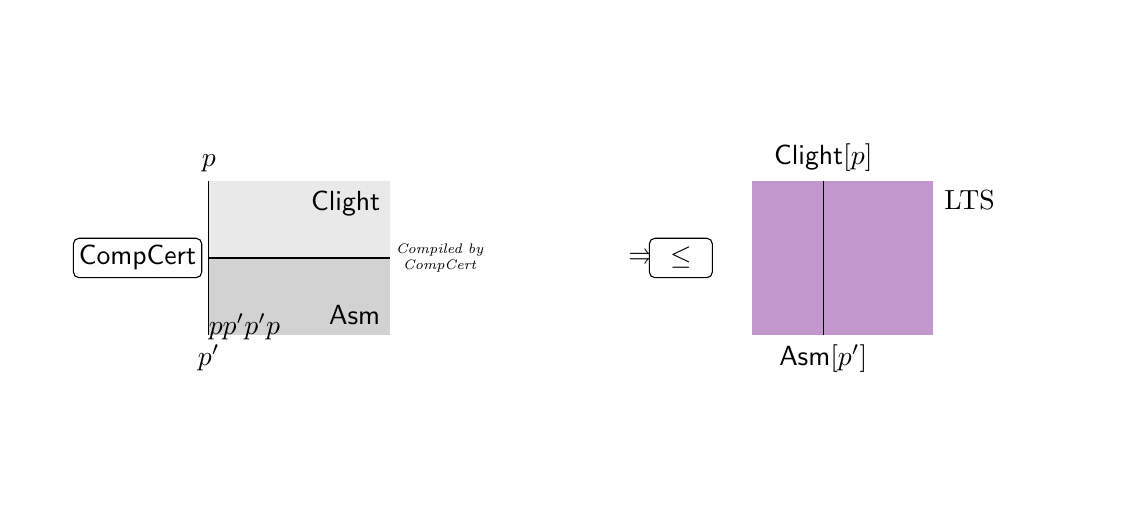
\begin{tikzpicture}[xscale=1.15,yscale=0.65]
      \path[gray\filltint,use as bounding box] (-2,-3) grid (+10,+6);

      \begin{scope}%[xshift=1cm]
        \coordinate (T) at (0,3);
        \coordinate (C) at (0,1.5);
        \coordinate (B) at (0,0);
        \coordinate (R) at (2,1.5);
        \simproof{(C)}{$\kw{CompCert}$}
        \draw
          (T) node[above] {$p$} --
          (B) node[below] {$p'$};
        {\tiny \it
        \drawsc
          (C) -- (R) node[right,align=center] {Compiled by \\ CompCert};
        }
        \node[below left] at (T -| R) {$\kw{Clight}$};
        \node[above left] at (B -| R) {$\kw{Asm}$};

        \begin{pgfonlayer}{background}
          \fill[lightgray\filltint] (T) rectangle (R);
          \fill[gray\filltint] (B) rectangle (R);
        \end{pgfonlayer}
      \end{scope}

      \note{\par
        For our purposes, \\
        CompCert is a compiler
        from Clight to assembly language, \\
        and it comes with a mechanized proof that
        when you compile $p$ to $p'$, \\
      }

      \only<2->{
      \note{
        the semantics of $p'$ \emph{refine} the semantics of $p$.

        In CompCert,
        this is established as \\
        a simulation between two transition systems. \\ }

      \node at (4,1.5) {$\Rightarrow$};

      \begin{scope}[xshift=6cm]
        \coordinate (T) at (0,3);
        \coordinate (C) at (0,1.5);
        \coordinate (B) at (0,0);
        \coordinate (BR) at (2,0);
        \simproof{(C)}{$\le$}
        \draw
          (T) node[above] {$\kw{Clight}[p]$} --
          (B) node[below] {$\kw{Asm}[p']$};

        \node[below left] at (T -| BR) {LTS};

        \begin{pgfonlayer}{background}
          \fill[ACMPurple\filltint] (T) rectangle (BR);
        \end{pgfonlayer}
      \end{scope}
      }
    \end{tikzpicture}
  \end{center}
  \vfill
  \begin{thebibliography}{0}
    \footnotesize
    \bibitem{compcomp}
      Xavier Leroy.
      \newblock Formal Verification of a Realistic Compiler.
      \newblock {\em Communications of the ACM, July 2009}
  \end{thebibliography}
\end{frame}
%}}}

\begin{frame}{Vertical Compositionality} %{{{
  \begin{center}
    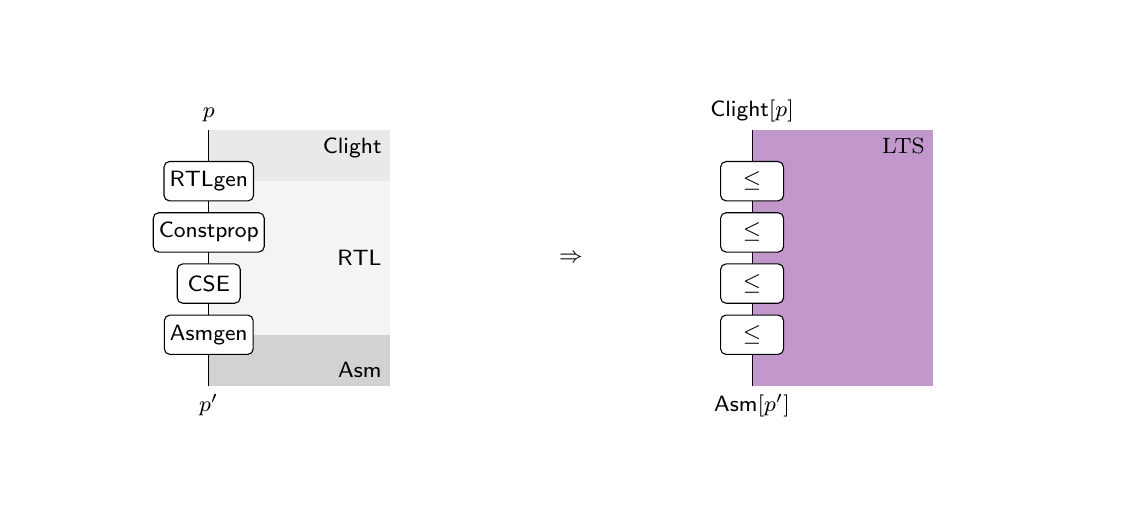
\begin{tikzpicture}[xscale=1.15,yscale=0.65]
      \path[gray\filltint,use as bounding box] (-2,-3) grid (+10,+6);
      \footnotesize

      \begin{scope}%[xshift=1cm]
        \coordinate (T) at (0,4);
        \coordinate (C) at (0,1.5);
        \coordinate (B) at (0,-1);
        \coordinate (R) at (2,1.5);
        \simproof{(0,3)}{$\kw{RTLgen}$}
        \simproof{(0,2)}{$\kw{Constprop}$}
        \simproof{(0,1)}{$\kw{CSE}$}
        \simproof{(0,0)}{$\kw{Asmgen}$}
        \draw
          (0,4) node[above] {$p$} --
          (0,-1) node[below] {$p'$};
%        \begin{scope}[every node/.style={right, align=center}]
%          \tiny \it
%          \drawsc (0,3) -- (0,3 -| R) node {Compiled by \\ \kw{RTLgen}};
%          \drawsc (0,2) -- (0,2 -| R) node {Compiled by \\ \kw{Constprop}};
%          \drawsc (0,1) -- (0,1 -| R) node {Compiled by \\ \kw{CSE}};
%          \drawsc (0,0) -- (0,0 -| R) node {Compiled by \\ \kw{Asmgen}};
%        \end{scope}
        \node[below left] at (0,4 -| R) {$\kw{Clight}$};
        \node[left] at (0,1.5 -| R) {$\kw{RTL}$};
        \node[above left] at (0,-1 -| R) {$\kw{Asm}$};

        \begin{pgfonlayer}{background}
          \fill[lightgray\filltint] (T) rectangle (0,3 -| R);
          \fill[lightgray!50!white\filltint] (0,3) rectangle (0,0 -| R);
          \fill[gray\filltint] (0,0) rectangle (0,-1 -| R);
        \end{pgfonlayer}
      \end{scope}

      \node at (4,1.5) {$\Rightarrow$};

      \begin{scope}[xshift=6cm]
        \coordinate (T) at (0,4);
        \coordinate (C) at (0,1.5);
        \coordinate (B) at (0,-1);
        \coordinate (BR) at (2,-1);
        \simproof{(0,3)}{$\le$}
        \simproof{(0,2)}{$\le$}
        \simproof{(0,1)}{$\le$}
        \simproof{(0,0)}{$\le$}
        \draw
          (T) node[above] {$\kw{Clight}[p]$} --
          (B) node[below] {$\kw{Asm}[p']$};

        \node[below left] at (T -| BR) {LTS};

        \begin{pgfonlayer}{background}
          \fill[ACMPurple\filltint] (T) rectangle (BR);
        \end{pgfonlayer}
      \end{scope}
    \end{tikzpicture}
  \end{center}
  \note{
    Because simulations are transitive, \\
    we can verify compilation passes in isolation, \\
    and combine the proofs \emph{vertically}
    to obtain the final theorem.
  }
  \vfill
  \begin{thebibliography}{0}
    \footnotesize
    \bibitem{compcomp}
      Xavier Leroy.
      \newblock Formal Verification of a Realistic Compiler.
      \newblock {\em Communications of the ACM, July 2009}
  \end{thebibliography}
\end{frame}
%}}}

\begin{frame}{Horizontal Compositionality} %{{{
  \note{
    Of course, C programs also decompose \emph{horizontally} into translation units.}
  \begin{center}
    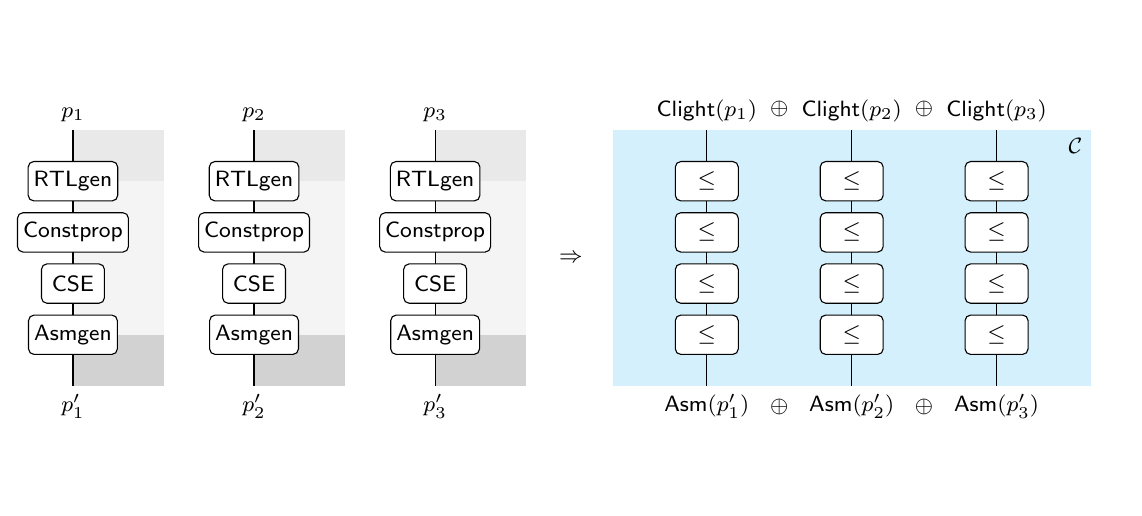
\begin{tikzpicture}[xscale=1.15,yscale=0.65]
      \path[gray\filltint,use as bounding box] (-2,-3) grid (+10,+6);
      \footnotesize

      % Syntax

      \begin{scope}[xshift=-1.5cm]
        \coordinate (T) at (0,4);
        \coordinate (C) at (0,1.5);
        \coordinate (B) at (0,-1);
        \coordinate (R) at (1,1.5);
        \simproof{(0,3)}{$\kw{RTLgen}$}
        \simproof{(0,2)}{$\kw{Constprop}$}
        \simproof{(0,1)}{$\kw{CSE}$}
        \simproof{(0,0)}{$\kw{Asmgen}$}
        \draw
          (0,4) node[above] {$p_1$} --
          (0,-1) node[below] {$p_1'$};
        \begin{pgfonlayer}{background}
          \fill[lightgray\filltint] (T) rectangle (0,3 -| R);
          \fill[lightgray!50!white\filltint] (0,3) rectangle (0,0 -| R);
          \fill[gray\filltint] (0,0) rectangle (0,-1 -| R);
        \end{pgfonlayer}
      \end{scope}

      \begin{scope}[xshift=0.5cm]
        \coordinate (T) at (0,4);
        \coordinate (C) at (0,1.5);
        \coordinate (B) at (0,-1);
        \coordinate (R) at (1,1.5);
        \simproof{(0,3)}{$\kw{RTLgen}$}
        \simproof{(0,2)}{$\kw{Constprop}$}
        \simproof{(0,1)}{$\kw{CSE}$}
        \simproof{(0,0)}{$\kw{Asmgen}$}
        \draw
          (0,4) node[above] {$p_2$} --
          (0,-1) node[below] {$p_2'$};
        \begin{pgfonlayer}{background}
          \fill[lightgray\filltint] (T) rectangle (0,3 -| R);
          \fill[lightgray!50!white\filltint] (0,3) rectangle (0,0 -| R);
          \fill[gray\filltint] (0,0) rectangle (0,-1 -| R);
        \end{pgfonlayer}
      \end{scope}

      \begin{scope}[xshift=+2.5cm]
        \coordinate (T) at (0,4);
        \coordinate (C) at (0,1.5);
        \coordinate (B) at (0,-1);
        \coordinate (R) at (1,1.5);
        \simproof{(0,3)}{$\kw{RTLgen}$}
        \simproof{(0,2)}{$\kw{Constprop}$}
        \simproof{(0,1)}{$\kw{CSE}$}
        \simproof{(0,0)}{$\kw{Asmgen}$}
        \draw
          (0,4) node[above] {$p_3$} --
          (0,-1) node[below] {$p_3'$};
        \begin{pgfonlayer}{background}
          \fill[lightgray\filltint] (T) rectangle (0,3 -| R);
          \fill[lightgray!50!white\filltint] (0,3) rectangle (0,0 -| R);
          \fill[gray\filltint] (0,0) rectangle (0,-1 -| R);
        \end{pgfonlayer}
      \end{scope}

      \note{\par
        To account for this, \\
      }

      \only<2->{

      \note{we can use a compositional semantics \\
        to model individual units and their interactions.

        If simulations compose both vertically and horizontally, \\
        the correctness theorem
        will be compatible with \emph{linking},
        but unfortunately, \\
        it's quite difficult to get simulations which compose in this way. \\
      }

      \node at (4,1.5) {$\Rightarrow$};

      \begin{scope}[xshift=5.5cm,xscale=0.8]
        \coordinate (TL) at (-1.3,4);
        \coordinate (BR) at (5.3,-1);
        \simproof{(0,3)}{$\le$}
        \simproof{(0,2)}{$\le$}
        \simproof{(0,1)}{$\le$}
        \simproof{(0,0)}{$\le$}
        \simproof{(2,3)}{$\le$}
        \simproof{(2,2)}{$\le$}
        \simproof{(2,1)}{$\le$}
        \simproof{(2,0)}{$\le$}
        \simproof{(4,3)}{$\le$}
        \simproof{(4,2)}{$\le$}
        \simproof{(4,1)}{$\le$}
        \simproof{(4,0)}{$\le$}
        \draw
          (0,4) node[above] {$\kw{Clight}(p_1)$} --
          (0,-1) node[below] {$\kw{Asm}(p_1')$};
        \draw
          (2,4) node[above] {$\kw{Clight}(p_2)$} --
          (2,-1) node[below] {$\kw{Asm}(p_2')$};
        \draw
          (4,4) node[above] {$\kw{Clight}(p_3)$} --
          (4,-1) node[below] {$\kw{Asm}(p_3')$};
        \node[above] at (1,4.1) {$\oplus$};
        \node[above] at (3,4.1) {$\oplus$};
        \node[below] at (1,-1.1) {$\oplus$};
        \node[below] at (3,-1.1) {$\oplus$};

        \node[below left] at (TL -| BR) {$\mathcal{C}$};

        \begin{pgfonlayer}{background}
          \fill[ACMLightBlue\filltint] (TL) rectangle (BR);
        \end{pgfonlayer}
      \end{scope}
      }
    \end{tikzpicture}
  \end{center}
  \vfill
  \uncover<2->{
  \begin{thebibliography}{0}
    \footnotesize
    \bibitem{compcomp}
      Gordon Steward, Lennart Beringer, Santiago Cuellar, Andrew W. Appel.
      \newblock Compositional CompCert.
      \newblock {\em POPL '2015}
  \end{thebibliography}
  }
\end{frame}
%}}}

\begin{frame}{SepCompCert} %{{{
  \note{The solution that is now used in CompCert
    \\ is to make the \emph{syntax} compositional, \\
    and to formulate the correctness theorem
    directly in terms of the \emph{linked} programs.
  }
%  \note<2->{\par
%    Most of the time,
%    compilers work function by function anyway, \\
%    so it doesn't really matter how these functions are \\
%    distributed across translation units.
%  }
  \begin{center}
    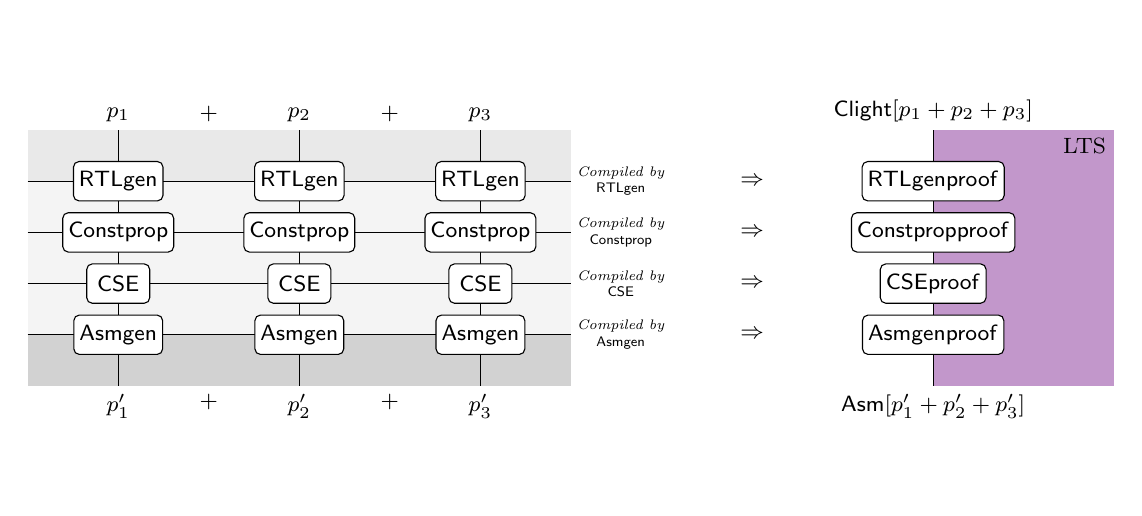
\begin{tikzpicture}[xscale=1.15,yscale=0.65]
      \path[gray\filltint,use as bounding box] (-2,-3) grid (+10,+6);
      \tikzset{xshift=0.5cm}
      \footnotesize

      % Syntax

      \begin{scope}[xshift=-1.5cm]
        \coordinate (T) at (0,4);
        \coordinate (C) at (0,1.5);
        \coordinate (B) at (0,-1);
        \coordinate (R) at (1,1.5);
        \simproof{(0,3)}{$\kw{RTLgen}$}
        \only<1->{\simproof{(0,2)}{$\kw{Constprop}$}}
        \only<1->{\simproof{(0,1)}{$\kw{CSE}$}}
        %\node<> at (0,2) {$\bullet$};
        %\node<> at (0,1) {$\bullet$};
        \simproof{(0,0)}{$\kw{Asmgen}$}
        \draw
          (0,4) node[above] {$p_1$} --
          (0,-1) node[below] {$p_1'$};
      \end{scope}

      \begin{scope}[xshift=0.5cm]
        \coordinate (T) at (0,4);
        \coordinate (C) at (0,1.5);
        \coordinate (B) at (0,-1);
        \coordinate (R) at (1,1.5);
        \simproof{(0,3)}{$\kw{RTLgen}$}
        \only<1->{\simproof{(0,2)}{$\kw{Constprop}$}}
        %\node<> at (0,2) {$\bullet$};
        \simproof{(0,1)}{$\kw{CSE}$}
        \simproof{(0,0)}{$\kw{Asmgen}$}
        \draw
          (0,4) node[above] {$p_2$} --
          (0,-1) node[below] {$p_2'$};
      \end{scope}

      \begin{scope}[xshift=+2.5cm]
        \coordinate (T) at (0,4);
        \coordinate (C) at (0,1.5);
        \coordinate (B) at (0,-1);
        \coordinate (R) at (1,1.5);
        \simproof{(0,3)}{$\kw{RTLgen}$}
        \simproof{(0,2)}{$\kw{Constprop}$}
        \only<1->{\simproof{(0,1)}{$\kw{CSE}$}}
        %\node<> at (0,1) {$\bullet$};
        \simproof{(0,0)}{$\kw{Asmgen}$}
        \draw
          (0,4) node[above] {$p_3$} --
          (0,-1) node[below] {$p_3'$};
      \end{scope}

      \node[above] at (-0.5,4) {$+$};
      \node[above] at (1.5,4) {$+$};
      \node[below] at (-0.5,-1) {$+$};
      \node[below] at (1.5,-1) {$+$};

      \begin{pgfonlayer}{background}
        \fill[lightgray\filltint] (-2.5,4) rectangle (0,3 -| R);
        \fill[lightgray!50!white\filltint] (-2.5,3) rectangle (0,0 -| R);
        \fill[gray\filltint] (-2.5,0) rectangle (0,-1 -| R);
      \end{pgfonlayer}

    \only<1->{
%      \note{\par To capture this, \\
%        we can introduce a compositional relation \\
%        between the source and target programs of each pass, \\
%        and show that if the \emph{linked} programs are related, \\
%      }
      \begin{scope}[every node/.style={align=center}]
        \tiny \it
        \drawsc (-2.5,3) -- (3.5,3) node[right] {Compiled by \\ $\kw{RTLgen}$};
        \drawsc (-2.5,2) -- (3.5,2) node[right] {Compiled by \\ $\kw{Constprop}$};
        \drawsc (-2.5,1) -- (3.5,1) node[right] {Compiled by \\ $\kw{CSE}$};
        \drawsc (-2.5,0) -- (3.5,0) node[right] {Compiled by \\ $\kw{Asmgen}$};
      \end{scope}
    }

    \only<1->{
      \node at (5.5,3) {$\Rightarrow$};
      \node at (5.5,2) {$\Rightarrow$};
      \node at (5.5,1) {$\Rightarrow$};
      \node at (5.5,0) {$\Rightarrow$};
      \begin{scope}[xshift=7.5cm]
        \coordinate (T) at (0,4);
        \coordinate (C) at (0,1.5);
        \coordinate (B) at (0,-1);
        \coordinate (BR) at (2,-1);
        \simproof{(0,3)}{$\kw{RTLgenproof}$}
        \simproof{(0,2)}{$\kw{Constpropproof}$}
        \simproof{(0,1)}{$\kw{CSEproof}$}
        \simproof{(0,0)}{$\kw{Asmgenproof}$}
        \draw
          (T) node[above] {$\kw{Clight}[p_1 + p_2 + p_3]$} --
          (B) node[below] {$\kw{Asm}[p_1' + p_2' + p_3']$};

        \node[below left] at (T -| BR) {LTS};

        \begin{pgfonlayer}{background}
          \fill[ACMPurple\filltint] (T) rectangle (BR);
        \end{pgfonlayer}
      \end{scope}
%      \note{then their semantics is related as well.}
    }
    \end{tikzpicture}
  \end{center}
  %\note<> {
  %  \par This method can even be extended to support \\
  %    mixed sets of optimizations \\
  %    across translations units.
  %}
  \vfill
  \uncover<1->{
  \begin{thebibliography}{0}
    \footnotesize
    \bibitem{compcomp}
      Jeehoon Kang, Yoonseung Kim, Chung-Kil Hur, Derek Dreyer, Viktor Vafeiadis.
      \newblock Lightweight Verification of Separate Compilation.
      \newblock {\em POPL '2016}
  \end{thebibliography}
  }
\end{frame}
%}}}

\begin{frame}{CompCertM} %{{{
  \note{Finally, in CompCertM, these approaches are combined \\ to build
    a verification platform for C and assembly, \\
    but because the final correctness theorem \\
    is expressed in terms of closed semantics, \\
    it's still difficult to use for heterogeneous verification.}

  \begin{center}
    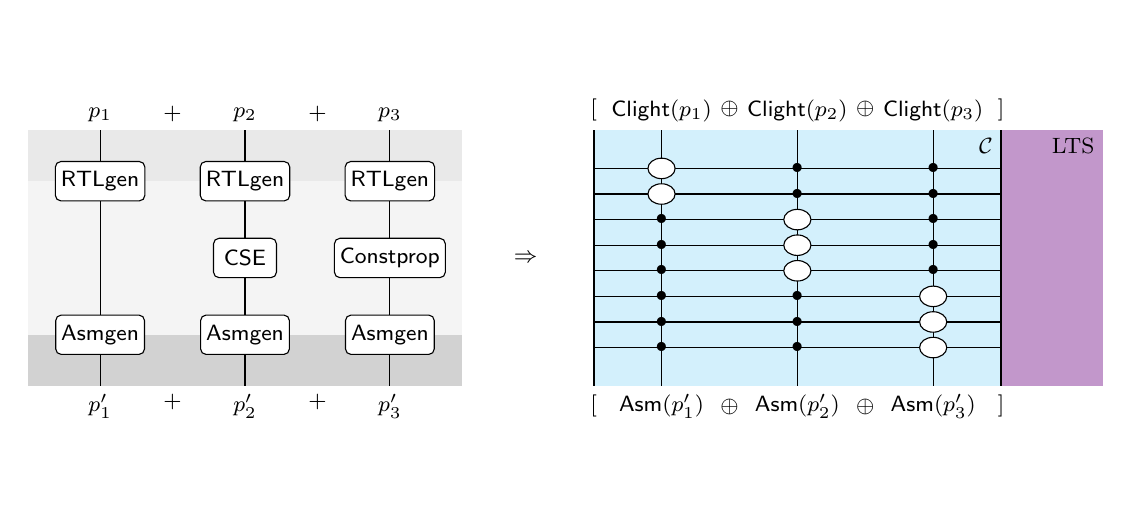
\begin{tikzpicture}[xscale=1.15,yscale=0.65]
      \path[gray\filltint,use as bounding box] (-2,-3) grid (+10,+6);
      \footnotesize

      % Syntax {{{

    \begin{scope}[xscale=0.8]
      \begin{scope}[xshift=-1.5cm]
        \coordinate (T) at (0,4);
        \coordinate (C) at (0,1.5);
        \coordinate (B) at (0,-1);
        \coordinate (R) at (1,1.5);
        \simproof{(0,3)}{$\kw{RTLgen}$}
        \simproof{(0,0)}{$\kw{Asmgen}$}
        \draw
          (0,4) node[above] {$p_1$} --
          (0,-1) node[below] {$p_1'$};
      \end{scope}

      \begin{scope}[xshift=0.5cm]
        \coordinate (T) at (0,4);
        \coordinate (C) at (0,1.5);
        \coordinate (B) at (0,-1);
        \coordinate (R) at (1,1.5);
        \simproof{(0,3)}{$\kw{RTLgen}$}
        \simproof{(0,1.5)}{$\kw{CSE}$}
        \simproof{(0,0)}{$\kw{Asmgen}$}
        \draw
          (0,4) node[above] {$p_2$} --
          (0,-1) node[below] {$p_2'$};
      \end{scope}

      \begin{scope}[xshift=+2.5cm]
        \coordinate (T) at (0,4);
        \coordinate (C) at (0,1.5);
        \coordinate (B) at (0,-1);
        \coordinate (R) at (1,1.5);
        \simproof{(0,3)}{$\kw{RTLgen}$}
        \simproof{(0,1.5)}{$\kw{Constprop}$}
        \simproof{(0,0)}{$\kw{Asmgen}$}
        \draw
          (0,4) node[above] {$p_3$} --
          (0,-1) node[below] {$p_3'$};
      \end{scope}

      \node[above] at (-0.5,4) {$+$};
      \node[above] at (1.5,4) {$+$};
      \node[below] at (-0.5,-1) {$+$};
      \node[below] at (1.5,-1) {$+$};

      \begin{pgfonlayer}{background}
        \fill[lightgray\filltint] (-2.5,4) rectangle (0,3 -| R);
        \fill[lightgray!50!white\filltint] (-2.5,3) rectangle (0,0 -| R);
        \fill[gray\filltint] (-2.5,0) rectangle (0,-1 -| R);
      \end{pgfonlayer}
    \end{scope}

      % }}}

      % Semantics {{{

      \node at (3.5,1.5) {$\Rightarrow$};

      \begin{scope}[xshift=5cm,xscale=0.75]
        \coordinate (TL) at (-1,4);
        \coordinate (BR) at (5,-1);

        \drawsc (-1.25,3.25 -| TL) -- (5.25,3.25 -| BR);
        \drawsc (-1.25,2.75 -| TL) -- (5.25,2.75 -| BR);
        \drawsc (-1.25,2.25 -| TL) -- (5.25,2.25 -| BR);
        \drawsc (-1.25,1.75 -| TL) -- (5.25,1.75 -| BR);
        \drawsc (-1.25,1.25 -| TL) -- (5.25,1.25 -| BR);
        \drawsc (-1.25,0.75 -| TL) -- (5.25,0.75 -| BR);
        \drawsc (-1.25,0.25 -| TL) -- (5.25,0.25 -| BR);
        \drawsc (-1.25,-.25 -| TL) -- (5.25,-.25 -| BR);
        \draw[thick]
          (TL) node[above] {$ [ $} --
          (TL |- BR) node[below] {$ [ $};
        \draw[thick]
          (TL -| BR) node[above] {$]$} --
          (BR) node[below] {$]$};
        \draw
          (0,4) node[above] {$\kw{Clight}(p_1)$} --
          (0,-1) node[below] {$\kw{Asm}(p_1')$};
        \draw
          (2,4) node[above] {$\kw{Clight}(p_2)$} --
          (2,-1) node[below] {$\kw{Asm}(p_2')$};
        \draw
          (4,4) node[above] {$\kw{Clight}(p_3)$} --
          (4,-1) node[below] {$\kw{Asm}(p_3')$};
        \node[above] at (1,4.1) {$\oplus$};
        \node[above] at (3,4.1) {$\oplus$};
        \node[below] at (1,-1.1) {$\oplus$};
        \node[below] at (3,-1.1) {$\oplus$};

        \osimproof{(0,3.25)}
        \osimproof{(0,2.75)}
        \node at (0,2.25) {$\bullet$};
        \node at (0,1.75) {$\bullet$};
        \node at (0,1.25) {$\bullet$};
        \node at (0,0.75) {$\bullet$};
        \node at (0,0.25) {$\bullet$};
        \node at (0,-.25) {$\bullet$};
        \osimproof{(2,2.25)}
        \osimproof{(2,1.75)}
        \osimproof{(2,1.25)}
        \node at (2,3.25) {$\bullet$};
        \node at (2,2.75) {$\bullet$};
        \node at (2,0.75) {$\bullet$};
        \node at (2,0.25) {$\bullet$};
        \node at (2,-.25) {$\bullet$};
        \osimproof{(4,0.75)}
        \osimproof{(4,0.25)}
        \osimproof{(4,-0.25)}
        \node at (4,3.25) {$\bullet$};
        \node at (4,2.75) {$\bullet$};
        \node at (4,2.25) {$\bullet$};
        \node at (4,1.75) {$\bullet$};
        \node at (4,1.25) {$\bullet$};

        \node[below left] at (TL -| BR) {$\mathcal{C}$};
        \node[below left] at (TL -| 6.5,0) {LTS};

        \begin{pgfonlayer}{background}
          \fill[ACMLightBlue\filltint] (TL) rectangle (BR);
          \fill[ACMPurple\filltint] (TL -| BR) rectangle (BR -| 6.5,0);
        \end{pgfonlayer}
      \end{scope}

      %}}}

    \end{tikzpicture}
  \end{center}
  \vfill
  \begin{thebibliography}{0}
    \footnotesize
    \bibitem{compcertm}
      Youngju Song, Minki Cho, Dongjoo Kim, Yonghyun Kim, Jeehoon Kang, Chung-Kil Hur.
      \newblock CompCertM: CompCert with C-Assembly Linking and Lightweight Modular Verification.
      \newblock {\em POPL '2019}
  \end{thebibliography}
\end{frame}
%}}}

\begin{frame}{CompCertO} %{{{
  \note{So that brings me to CompCertO, \\
    which uses compositional semantics
    with an open correctness theorem, \\
    but which avoids making simulations too complex, \\
    by making them more general instead.
  }

  \begin{center}
    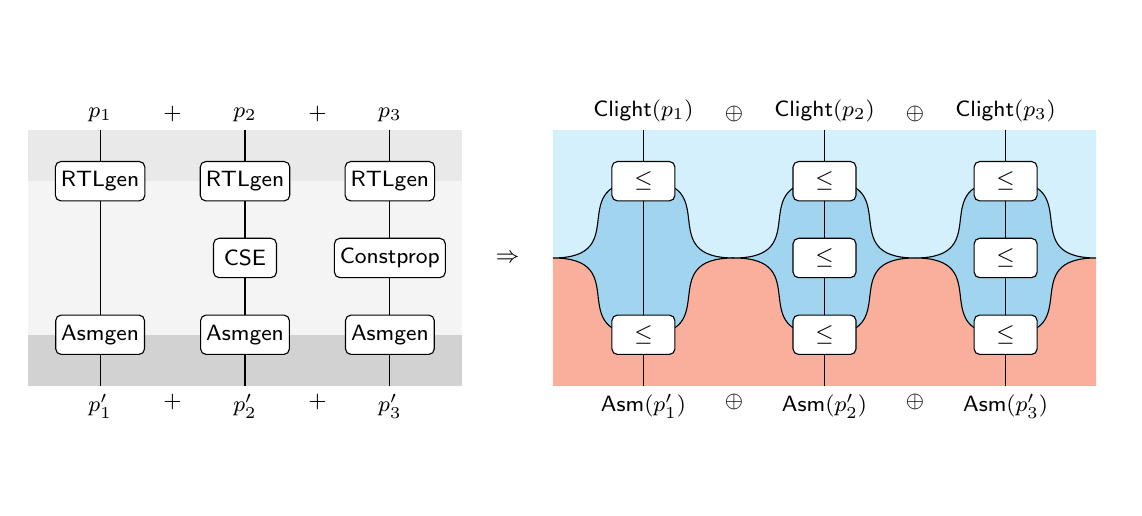
\begin{tikzpicture}[xscale=1.15,yscale=0.65]
      \path[gray\filltint,use as bounding box] (-2,-3) grid (+10,+6);
      \footnotesize

      % Syntax {{{

    \begin{scope}[xscale=0.8]
      \begin{scope}[xshift=-1.5cm]
        \coordinate (T) at (0,4);
        \coordinate (C) at (0,1.5);
        \coordinate (B) at (0,-1);
        \coordinate (R) at (1,1.5);
        \simproof{(0,3)}{$\kw{RTLgen}$}
        \simproof{(0,0)}{$\kw{Asmgen}$}
        \draw
          (0,4) node[above] {$p_1$} --
          (0,-1) node[below] {$p_1'$};
      \end{scope}

      \begin{scope}[xshift=0.5cm]
        \coordinate (T) at (0,4);
        \coordinate (C) at (0,1.5);
        \coordinate (B) at (0,-1);
        \coordinate (R) at (1,1.5);
        \simproof{(0,3)}{$\kw{RTLgen}$}
        \simproof{(0,1.5)}{$\kw{CSE}$}
        \simproof{(0,0)}{$\kw{Asmgen}$}
        \draw
          (0,4) node[above] {$p_2$} --
          (0,-1) node[below] {$p_2'$};
      \end{scope}

      \begin{scope}[xshift=+2.5cm]
        \coordinate (T) at (0,4);
        \coordinate (C) at (0,1.5);
        \coordinate (B) at (0,-1);
        \coordinate (R) at (1,1.5);
        \simproof{(0,3)}{$\kw{RTLgen}$}
        \simproof{(0,1.5)}{$\kw{Constprop}$}
        \simproof{(0,0)}{$\kw{Asmgen}$}
        \draw
          (0,4) node[above] {$p_3$} --
          (0,-1) node[below] {$p_3'$};
      \end{scope}

      \node[above] at (-0.5,4) {$+$};
      \node[above] at (1.5,4) {$+$};
      \node[below] at (-0.5,-1) {$+$};
      \node[below] at (1.5,-1) {$+$};

      \begin{pgfonlayer}{background}
        \fill[lightgray\filltint] (-2.5,4) rectangle (0,3 -| R);
        \fill[lightgray!50!white\filltint] (-2.5,3) rectangle (0,0 -| R);
        \fill[gray\filltint] (-2.5,0) rectangle (0,-1 -| R);
      \end{pgfonlayer}
    \end{scope}

      % }}}

      \node at (3.3,1.5) {$\Rightarrow$};

      % Semantics {{{

    \begin{scope}[xshift=6.3cm,xscale=1]
    \tikzset{to path={
      .. controls ($(\tikztostart)!0.9!(\tikztostart -| \tikztotarget)$)
              and ($(\tikztotarget)!0.9!(\tikztotarget -| \tikztostart)$) ..
      (\tikztotarget) \tikztonodes}}

      \begin{scope}[xshift=-1.5cm]
        \coordinate (T1) at (0,4);
        \coordinate (B1) at (0,-1);
        \coordinate (L1) at (-1,1.5);
        \coordinate (R1) at (1,1.5);
        \coordinate (N11) at (0,3);
        \coordinate (N14) at (0,0);
        \simproof{(N11)}{$\le$}
        \simproof{(N14)}{$\le$}
        \draw
          (T1) node[above] {$\kw{Clight}(p_1)$} --
          (B1) node[below] {$\kw{Asm}(p_1')$};
      \end{scope}

      \begin{scope}[xshift=0.5cm]
        \coordinate (T2) at (0,4);
        \coordinate (B2) at (0,-1);
        \coordinate (L2) at (-1,1.5);
        \coordinate (R2) at (1,1.5);
        \coordinate (N21) at (0,3);
        \coordinate (N22) at (0,1.5);
        \coordinate (N24) at (0,0);
        \simproof{(N21)}{$\le$}
        \simproof{(N22)}{$\le$}
        \simproof{(N24)}{$\le$}
        \draw
          (T2) node[above] {$\kw{Clight}(p_2)$} --
          (B2) node[below] {$\kw{Asm}(p_2')$};
        %\drawsc (L2) to (N22) to (R2);
      \end{scope}

      \begin{scope}[xshift=2.5cm]
        \coordinate (T3) at (0,4);
        \coordinate (B3) at (0,-1);
        \coordinate (L3) at (-1,1.5);
        \coordinate (R3) at (1,1.5);
        \coordinate (N31) at (0,3);
        \coordinate (N33) at (0,1.5);
        \coordinate (N34) at (0,0);
        \simproof{(N31)}{$\le$}
        \simproof{(N33)}{$\le$}
        \simproof{(N34)}{$\le$}
        \draw
          (T3) node[above] {$\kw{Clight}(p_3)$} --
          (B3) node[below] {$\kw{Asm}(p_3')$};
        %\drawsc (L3) to (N33) to (R3);
      \end{scope}

      \node[above] at (-0.5,4) {$\oplus$};
      \node[above] at (1.5,4) {$\oplus$};
      \node[below] at (-0.5,-1) {$\oplus$};
      \node[below] at (1.5,-1) {$\oplus$};

      \begin{pgfonlayer}{background}
        \fill[ACMLightBlue\filltint]
          (T1) -| (L1) to (N11) to (R1) --
                  (L2) to (N21) to (R2) --
                  (L3) to (N31) to (R3) |- cycle;
        \fill[ACMRed\filltint]
          (B1) -| (L1) to (N14) to (R1) --
                  (L2) to (N24) to (R2) --
                  (L3) to (N34) to (R3) |- cycle;
        \begin{scope}[every path/.style={fill=ACMBlue\filltint}]
          \draw (L1) to (N11) to (R1) to (N14) to cycle;
          \draw (L2) to (N21) to (R2) to (N24) to cycle;
          \draw (L3) to (N31) to (R3) to (N34) to cycle;
        \end{scope}
      \end{pgfonlayer}
    \end{scope}

      %}}}

    \end{tikzpicture}
  \end{center}
\end{frame}
%}}}

\section{Overview of CompCertO}

  \note{So the main ingredients
    of our semantics framework are} 

\begin{frame}{Ingredients}
  \centering
  \begin{tabular}{c@{\qquad\qquad}c@{\qquad\qquad}l}
    \begin{tile}{scale=1.2,baseline=-1mm}
      \fillboth{ACMBlue\filltint}
      \node (A) at (C) {$A$};
    \end{tile} &
    $A$ &
    Language interfaces
    \note{First, \emph{language interfaces} specify
      how components call each other \\
      at a given level of abstraction.}
    \pause
    \vspace{2em} \\
    \begin{tile}{scale=1.2,baseline=-1mm}
      \fillleft{ACMLightBlue\filltint}
      \fillright{ACMBlue\filltint}
      \draw (T) node[above,overlay] {\footnotesize $L$} --
            (B) node[below,overlay] {\footnotesize $L$};
      \node (A) at (-0.5,0) {$A$};
      \node at (+0.5,0) {$B$};
    \end{tile} &
    $L : A \rightarrow B$ &
    Open transition system
    \note<2->{\par They are used to parametrize our transition systems \\
      for their \emph{outgoing} calls and their \emph{incoming} calls.}
    \pause
    \vspace{2em} \\
    \begin{tile}{scale=1.2,baseline=-1mm}
      \filltop{ACMOrange\filltint}
      \fillbot{ACMRed\filltint}
      \drawsc (L) node[left,overlay] {$\mathbb{R}$} --
              (R) node[right,overlay] (SC) {$\mathbb{R}$};
      \node at (0,+0.75) {$A$};
      \node at (0,-0.75) {$B$};
    \end{tile} &
    $\mathbb{R} : A \Leftrightarrow B$ &
    Simulation conventions
    \note<3->{\par Finally,
      \emph{simulation conventions}
      are used to relate component interactions \\
      between the source level and the target level.}
  \end{tabular}
\end{frame}

\begin{frame}{Proof techniques}
  \centering
  \begin{tabular}{c@{\qquad\quad}c@{\qquad\qquad}l}
    \begin{tile}{scale=1.2,baseline=-1mm}
      \draw (T) node[above,overlay] {\footnotesize $L_1$} -- (B)
                node[below,overlay] {\footnotesize $L_2$};
      \drawsc (L) node[left] {$\mathbb{R}$}
           -- (R) node[right] {$\mathbb{S}$};
      \simproof{(C)}{$\le$}
      \begin{pgfonlayer}{tint}
        \fill[ACMLightBlue\filltint] (TLC) rectangle (C.center);
        \fill[ACMOrange\filltint] (L) rectangle (B);
        \fill[ACMBlue\filltint] (T) rectangle (R);
        \fill[ACMRed\filltint] (C.center) rectangle (BRC);
      \end{pgfonlayer}
    \end{tile} &
    $L_1 \le_{\mathbb{R} \rightarrow \mathbb{S}} L_2$ &
    Simulation proofs
    \note{For each simulation proof in CompCert, \\
      we can choose appropriate simulation conventions,}
    \pause
    \vspace{2em} \\
    \begin{tile}{scale=1.2,baseline=-1mm}
      \filltop{ACMLightBlue\filltint}
      \fillbot{ACMRed\filltint}
      \drawsc (L) node[left,overlay] {$\mathbb{R}$} --
              (R) node[right,overlay] {$\mathbb{R}'$};
      \simproof{(C)}{$\sqsubseteq$}
    \end{tile} &
    $\mathbb{R} \sqsubseteq \mathbb{R}'$ &
    Simulation convention refinement
    \note<1->{\par but then
      the challenge is to derive
      a uniform simulation convention for the whole compiler. \\ }
    \note<2->{
      Our approach is to use a notion of
      \emph{simulation convention refinement}, and \\ }
    \pause
    \vspace{2em} \\
    \begin{tile}{scale=1.2,baseline=-1mm}
      \drawsc (L) node[left,overlay] {$\cc{C}{L}$}
        -- (R) node[right,overlay] {$\cc{C}{L}$};
      \drawsc (TL) node[left,overlay] {$\kw{inj}$}
        -- (TLB) -- (C) -- (BRB)
        -- (BR) node[right,overlay] {$\kw{inj}$};
      \filltop{ACMLightBlue\filltint}
      \fillbot{ACMBlue\filltint}
      \node[below left,inner sep=1pt] at (TRC) {$\mathcal{C}$};
      \node[above right,inner sep=1pt] at (BLC) {$\mathcal{L}$};
    \end{tile} &
    $\kw{inj} \cdot \cc{C}{L} \sqsubseteq \cc{C}{L} \cdot \kw{inj}$ &
    Simulation convention algebra
    \note<3->{
      to develop a simulation convention \emph{algebra}, \\
      which we use to establish and combine refinement properties \\
      like the one I've shown here.}
  \end{tabular}
\end{frame}

\begin{frame}{Correctness Proof} %{{{
  \centering
  \note{Our compiler correctness proof \\
    is built by assembling these kinds of two-dimensional \emph{tiles}.
      \\ \par
    We use the proofs of CompCert passes with almost no changes, \\
    and we obtain compositionality \\
    by building a sort of harness around them.
  }
  \figsize
  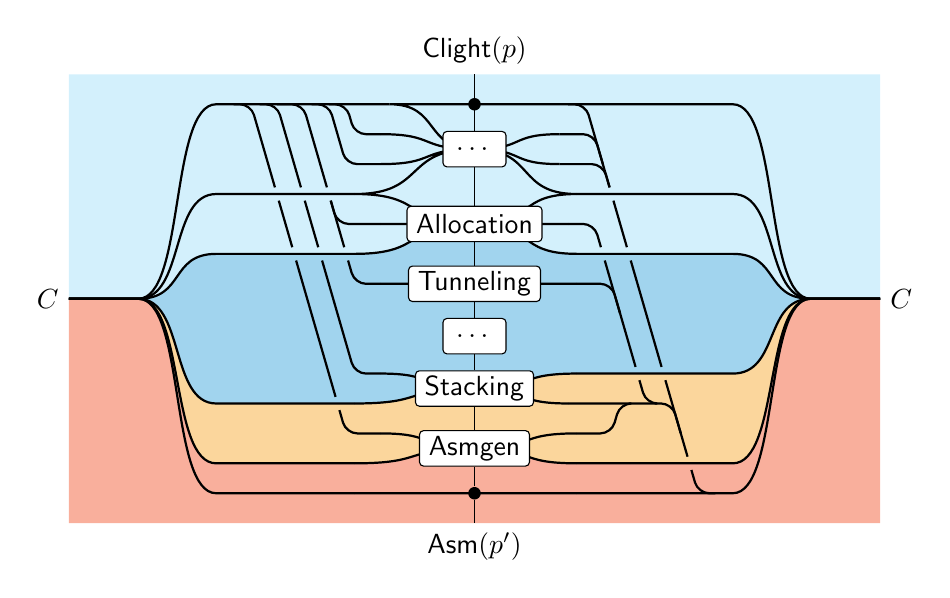
\begin{tikzpicture}[yscale=0.38,thick]
    \tikzset{to path={
      .. controls ($(\tikztostart)!\stens!(\tikztostart -| \tikztotarget)$)
              and ($(\tikztotarget)!\stens!(\tikztotarget -| \tikztostart)$) ..
      (\tikztotarget) \tikztonodes}}

    % Refinement of the incoming convention
    \begin{scope}[xshift=1.3cm,xscale=0.11]

      % Fan out from here
      \coordinate (RB) at (27,7.5);
      \coordinate (R) at (35,7.5);

      \draw (-1,14) coordinate (XI1) -- (18,14) to (RB) -- (R);
      \draw (0,11) coordinate (AI1) -- (18,11) to (RB) -- (R);
      \draw (0, 9) coordinate (AI3) -- (18, 9) coordinate (CLI) to (RB) -- (R);
      \draw (0, 5) coordinate (SI1) -- (18, 5) coordinate (LMI) to (RB) -- (R);
      \draw (0, 2) coordinate (GI2) -- (18, 2) coordinate (MAI) to (RB) -- (R);
      \draw (0, 1) coordinate (RaI) -- (18, 1) to (RB) -- (R);
      \node[right] at (R) {$\mathbb{C}$};

      % From now on we will use nodes as gaps around crossings
      \tikzset{rounded corners,every node/.style={inner sep=2pt}};

      % The vainj across
      \node (C1) at (4,11) {};
      \node (C2) at (6, 9) {};
      \node (C3) at (10,5) {};
      \node (C4) at (13,2) {};
      \draw (XI1) -- (1,14) -- (C1) -- (C2) -- (C3) -- (C4) -- (14,1) -- (16,1);

      % Spikes off of vainj
      \draw (-2,13) coordinate (XI2) -- (2,13) -- (3,12); % inj
      \draw (-2,12) coordinate (XI3) -- (3,12) -- (C1); % vainj
      \draw (-1, 4) coordinate (SI2) -- (11,4) -- (12,3); % inj

      % Spikes off of that last inj
      \node (C5) at (3,9) {};
      \node (C6) at (7,5) {};
      \draw (-1,10) coordinate (AI2) -- (2,10) -- (C5) -- (C6) -- (8,4) -- (9,4); % ext
      \draw (0, 8) coordinate (TI) -- (4,8) -- (5,7); % ext
      \draw (0, 3) coordinate (GI1) -- (4,3) -- (5,4) -- (6,4); % ext
    \end{scope}

    % Refinement of the outgoing convention
    \begin{scope}[xshift=-1.52cm,xscale=-0.11]

      % Fan out from here
      \coordinate (LB) at (25,7.5);
      \coordinate (L) at (33,7.5);

      \draw (-4,14) coordinate (XO1) -- (16,14) to (LB) -- (L);
      \draw (0,11) coordinate (AO1) -- (16,11) to (LB) -- (L);
      \draw (0, 9) coordinate (AO3) -- (16, 9) coordinate (CLO) to (LB) -- (L);
      \draw (0, 4) coordinate (SO1) -- (16, 4) coordinate (LMO) to (LB) -- (L);
      \draw (0, 2) coordinate (GO2) -- (16, 2) coordinate (MAO) to (LB) -- (L);
      \draw (0, 1) coordinate (RaO) -- (16, 1) to (LB) -- (L);
      \node[left] at (L) {$\mathbb{C}$};

      % From now on we will use nodes as gaps around crossings
      \tikzset{rounded corners,every node/.style={inner sep=2pt}};

      % Asmgen
      \node (D1) at ( 2, 4) {};
      \node (D2) at ( 7, 9) {};
      \node (D3) at ( 9,11) {};
      \draw (-3, 3) coordinate (GO1) -- (1, 3) -- (D1) -- (D2) -- (D3) -- (12,14) -- (14,14);

      % Stacking
      \node (D5) at ( 4, 9) {};
      \node (D6) at ( 6,11) {};
      \draw (-3, 5) coordinate (SO2) -- (0, 5) -- (D5) -- (D6) -- (9,14) -- (11,14);

      % Tunneling
      \node (D7) at ( 1, 9) {};
      \node (D8) at ( 3,11) {};
      \draw (-3, 8) coordinate (TO)  -- (0, 8) -- (D7) -- (D8);

      % Allocation
      \draw (-3,10) coordinate (AO2) -- (2,10) -- (D8) -- ( 6,14) -- ( 9,14);

      % Frontend
      \draw (-3,12) coordinate (XO3) -- (1,12) -- ( 3,14) -- ( 5,14);
      \draw (-3,13) coordinate (XO2) -- (0,13) -- ( 1,14) -- ( 3,14);
    \end{scope}

    % Nodes
    \begin{scope}
      \begin{pgfonlayer}{nodes}
        \begin{scope}[every node/.style={draw,fill=white,rounded corners=0.5mm,minimum height=0.45cm,inner ysep=0pt}]
          \node[minimum width=0.8cm] (X) at (0,12.5) {\ldots};
          \node (A) at (0,10) {$\kw{Allocation}$};
          \node (T) at (0,8) {$\kw{Tunneling}$};
          \node[minimum width=0.8cm] (C) at (0,6.25) {\ldots};
          \node (S) at (0,4.5) {$\kw{Stacking}$};
          \node (G) at (0,2.5) {$\kw{Asmgen}$};
        \end{scope}
        \begin{scope}[every node/.style={fill=black,circle,inner sep=1.6pt}]
          \node (RC) at (0,14) {};
          \node (RA) at (0,1) {};
        \end{scope}
      \end{pgfonlayer}
    \end{scope}

    \draw[thin]
      (0,15) coordinate (SP) node[above] {$\kw{Clight}(p)$} --
      (X) -- (A) -- (T) -- (C) -- (S) -- (G) -- (RA) --
      (0,0) coordinate (TP) node[below] {$\kw{Asm}(p')$};

    \draw
      (XI1) to (RC.center) to (XO1)
               (X.center) to (XO1)
      (XI2) to (X.center) to (XO2)
      (XI3) to (X.center) to (XO3)
      (AI1) to (X.center) to (AO1)
      (AI1) to (A.center) to (AO1)
      (AI2) to (A.center) to (AO2)
      (AI3) to (A.center) to (AO3)
      (TI)  to (T.center) to (TO)
      (SI1) to (S.center) to (SO1)
      (SI2) to (S.center) to (SO2)
      (GI1) to (G.center) to (GO1)
      (GI2) to (G.center) to (GO2)
      (RaI) to (RA.center) to (RaO);

    % Extra simulation convention labels
%    \tiny
%    \path[every node/.style={inner sep=0.8pt}]
%      (XI2) node[above] {$\kw{inj}$}
%      (XI3) node[above] {$\kw{vainj}$}
%      (GI1) node[above] {$\kw{ext}$}
%      (SI2) node[above] {$\kw{inj}$}
%      (TI)  node[above] {$\kw{ext}$}
%      (AI2) node[above] {$\kw{ext}$}
%      (XO2) node[above] {$\kw{inj}$}
%      (XO3) node[above] {$\kw{vainj}$}
%      (AO2) node[above] {$\kw{ext}$}
%      (TO) node[above] {$\kw{ext}$}
%      (SO2) node[above] {$\kw{injp}$}
%      (GO1) node[above] {$\kw{ext}$};

    % Region coloring
    \begin{pgfonlayer}{tint}
      \fill[ACMLightBlue\filltint]
        (R) -- (RB) to (CLI) --
        (AI3) to (A.center) to (AO3) --
        (CLO) to (LB) -- (L) |- (SP) -| cycle;
      \fill[ACMBlue\filltint]
        (RB) to
        (CLI) -- (AI3) to (A.center) to (AO3) -- (CLO) to (LB) to
        (LMO) -- (SO1) to (S.center) to (SI1) -- (LMI) to cycle;
      \fill[ACMOrange\filltint]
        (LB) to
        (LMO) -- (SO1) to (S.center) to (SI1) -- (LMI) to (RB) to
        (MAI) -- (GI2) to (G.center) to (GO2) -- (MAO) to cycle;
      \fill[ACMRed\filltint]
        (R) -- (RB) to
        (MAI) -- (GI2) to (G.center) to (GO2) -- (MAO) to (LB) --
        (L) |- (TP) -| cycle;
    \end{pgfonlayer}

  \end{tikzpicture}
\end{frame}
%}}}

\begin{frame}{Towards heterogeneous verification} %{{{
  \centering
  \note<1->{Going forward, \\
    we want to use these techniques \\
    for heterogeneous verification.

    In our driver example, \\
    the heterogeneous system would have a specification $\sigma$, \\
    which is decomposed into a hardware model
    and a code specification. \\
    This code is implemented and compiled with CompCert, \\
    to build a system which
    implements $\sigma$, \\
    modulo the C calling convention.}

  \note<2>{\par
    We can then link client code with the proof \\
    in the way that I've depicted here.}

  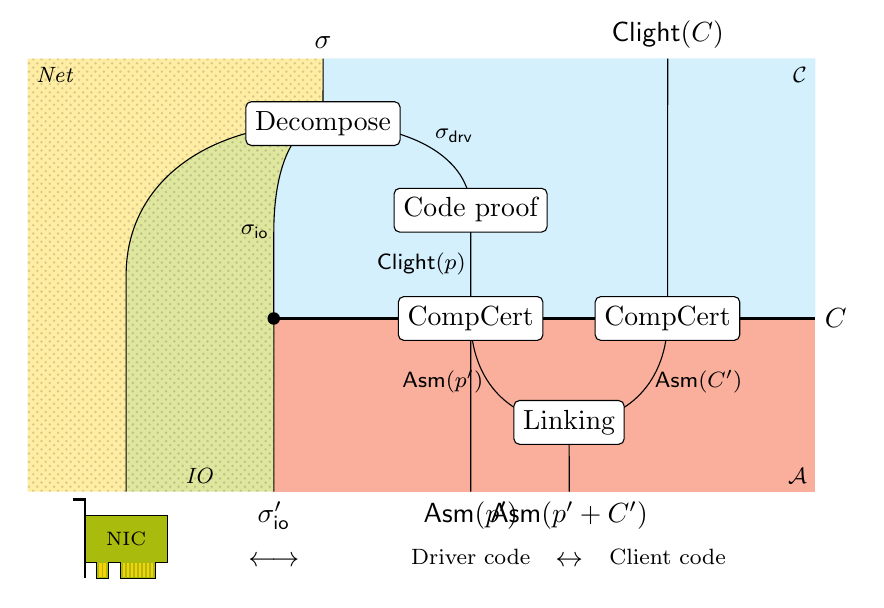
\begin{tikzpicture}[xscale=2.5,yscale=1.1]
    \tikzset{to path={
      .. controls ($(\tikztostart)!\stens!(\tikztostart -| \tikztotarget)$)
              and ($(\tikztotarget)!\stens!(\tikztostart -| \tikztotarget)$) ..
      (\tikztotarget) \tikztonodes}}

    \begin{pgfonlayer}{nodes}
      \begin{scope}[every node/.style={draw,fill=white,rounded corners=2pt}]
        \tikzset{text height=0.7em,text depth=0.5ex}
        \path
          (0.25,1.5) coordinate (NIC1)
          (1,2) coordinate (IO1)
          (1.25,3.25) coordinate (Def) node {Decompose}
          (2,2.25) coordinate (CP) node {Code proof}
          (2,1) coordinate (T1) node {CompCert};
        \path<2->
          (3,1) coordinate (T2) node {CompCert}
          (2.5,-0.2) coordinate (LK) node {Linking};
      \end{scope}
      \path (1,1) coordinate (IO) node [fill=black,circle,inner sep=1.6pt] {};
    \end{pgfonlayer}

    % Boundary
    \begin{scope}
      % Corners
      \path (-0.25, 4)       coordinate (ULC)
            ( 2,   -1)       coordinate (LRC)
            ($(ULC -| LRC)$) coordinate (URC)
            ($(ULC |- LRC)$) coordinate (LLC);

      % Source transition systems
      \path ($(Def |- ULC)$) coordinate (Spec) node[above] {$\sigma$};
      \path<2-> ($(T2 |- ULC)$) coordinate (CC);
      \path<2-> (CC) node[above,overlay] {$\kw{Clight}(C)$};

      % Target transition systems
      \path ($(NIC1 |- LRC)$) coordinate (NIC2) pic[yshift=-6mm] {l-nic}; % node[below] {$\sigma_\kw{NIC}$};
      \path ($(IO1 |- LRC)$) coordinate (IO2) node[below] {$\sigma_\kw{io}'$};
      \path ($(T1 |- IO2)$) coordinate (DRV2); \node<1>[below] at (DRV2) {$\kw{Asm}(p')$};
      \path<2-> ($(LK |- LRC)$) coordinate (CD2) node[below] {$\kw{Asm}(p' + C')$};

      % Extra labels
      \node[below,yshift=-7mm] at (IO2) {$\longleftrightarrow$};
      \node[below,yshift=-6mm] at (DRV2) {\footnotesize Driver code};
      \node<2->[below,yshift=-7mm] at (CD2) {$\leftrightarrow$};
      \node<2->[below,yshift=-6mm] at (T2 |- IO2) {\footnotesize Client code};

      % Simulation convention
      \path (3.75,1) coordinate (C) node[right] {$\mathbb{C}$};
    \end{scope}

    % Transition systems
    \begin{scope}[inner sep=1.6pt]
      \footnotesize
      \draw (Def) to (NIC1) -- (NIC2);
      \draw (Def) to node[above right] {$\sigma_\kw{drv}$} (CP.center)
        (CP) -- node[left] {$\kw{Clight}(p)$} (T1);
      \draw<2-> (T1)
        (LK.center) to node[left,pos=0.6] {$\kw{Asm}(p')$} (T1.center)
        (LK) -- (CD2);
      \draw<1> (T1) -- (DRV2);
      \draw<2-> (CC) -- (T2)
        (LK.center) to node[right,pos=0.6] {$\kw{Asm}(C')$} (T2.center);
      \draw (Spec)
        -- (Def) to (IO1) node[left] {$\sigma_\kw{io}$}
        -- (IO)
        -- (IO2);
    \end{scope}

    % Simulation convention
    \draw[thick] (IO) -- (C);

    % Colors
    \begin{pgfonlayer}{tint}
      \begin{scope}[every node/.style={black}]
        \footnotesize
        \fill[ACMYellow\filltint] (ULC) -- (Spec) -- (Def)
          to (NIC2) -| (ULC);
        \fill[ACMGreen\filltint]
          (Def) to (NIC1) |- (IO2)
          (Def) to (IO1) -- (IO2);
        \fill[pattern=crosshatch dots,opacity=.15]
          (ULC) -- (Spec) -- (Def) to (IO1) -- (IO2) -| cycle;
        \fill[ACMLightBlue\filltint]
          (Spec) -- (Def) to (IO1) -- (IO) -- (C) |- cycle;
        \fill[ACMRed\filltint] (IO2) rectangle (C);
        \node[below right] at (ULC) {$\li{Net}$};
        \node[above] at ($(NIC2)!0.5!(IO2)$) {$\li{IO}$};
        \node[below left] at ($(Spec -| C)$) {$\mathcal{C}$};
        \node[above left] at ($(IO2 -| C)$) {$\mathcal{A}$};
      \end{scope}
    \end{pgfonlayer}
  \end{tikzpicture}
\end{frame}
%}}}

\begin{frame}
  \centering \Large See you at the poster session!
  \note{So that concludes my talk, \\
    I hope it encourages you to check out our paper and longer video, \\
    and to chat with us at the poster sessions.}
\end{frame}

\iffalse

\section*{Introduction} %{{{

\begin{frame}{End-to-end verification of heterogeneous systems} %{{{

  \centering
  \begin{tikzpicture}[xscale=3,yscale=1.8]
    % Set a draw color to use as guide
    % When invisible, it ensures the bounding box is fixed
    \path (-0.5,-0.5) grid (2.5,2.5);

    % We use the following style to introduce invisible nodes to give
    % pictures a "shape" we can use to anchor edges
    \tikzset{blob/.style={
      ellipse,
      %fill=lightgray,
      minimum height=1cm,
      minimum width=1.8cm,
      outer sep=1ex,
    }}

    % For programs, we use text labels with a "C" blue background
    \tikzset{cprog/.style={
      draw,
      fill=ACMLightBlue\filltint,
      rounded corners,
      minimum height=1.6em,
      outer sep=1ex,
    }}

    % 1. We will consider what it means to have a certified web server
    \node[cprog] (WEB) at (1,2) {Web server};

    % 2. A good specification really must model the network and file system
    \only<2->{
      \node[blob] (FS) at (0,2) {}; \pic at (FS.center) {filesys};
      \node[blob] (NET) [cloud,aspect=2,draw,fill=lightgray,inner sep=0.5mm]
        at (2,2) {\scriptsize Network};
      \draw[<->] (FS) -- (WEB);
      \draw[<->] (WEB) -- (NET);
    }

    % 3. But those things are really abstractions, to really verify
    % things we must model the system that actually runs
    \only<3->{
      \node[blob] (HDD) at (0,0) {}; \pic<2-> at (HDD.center) {hdd};
      \node[blob] (CPU) at (1,0) {}; \pic<2-> at (CPU.center) {cpu};
      \node[blob] (NIC) at (2,0) {}; \pic<2-> at (NIC.center) {nic};
      %\node[blob] (ETH) at (3,0) {}; \pic at (ETH.center) {eth};
      \draw[<->] (HDD) -- (CPU);
      \draw[<->] (CPU) -- (NIC);
    }

    % 4. A key question is the relationship between the two
    \only<4->{
      \draw[double equal sign distance,Implies-Implies] (FS) -- (HDD);
      \draw[double equal sign distance,Implies-Implies] (WEB) -- (CPU);
      \draw[double equal sign distance,Implies-Implies] (NET) -- (NIC);
    }

    % 5. In-between, there is a lot of code involved
    \node<5-6>[align=center,fill=white,ellipse] (OS) at (1,1.05)
      {Operating system, \\ compilers, etc.};
    % We do operating systems and compilers, among other things
    \node<7-8> at (1,1.05) {\includegraphics[scale=0.2]{flint-banner}};

    % Thankfully, many of these things have been verified
    \tikzset{checkmark/.style={
      text=ACMGreen,
      node contents=\checkmark,
      overlay,
    }}
    \path<6-7>
      (FS.north east) node[checkmark]
      (WEB.north east) node[checkmark]
      (NET.east) node[right,checkmark]
      (CPU.south east) node[checkmark]
      (OS.north east) node[checkmark];

    % What we need is a glue
    \begin{pgfonlayer}{background}
      \node<8->[overlay,
          ellipse,
          cloud puffs=16,
          minimum height=7cm,
          minimum width=10cm,
          fill=gray!5]
        (GLUE) at (1,1) {};
      \node<8>[overlay,text=ACMGreen] at (GLUE.east) {\Huge \checkmark};
    \end{pgfonlayer}

    \node<9->[ellipse,fill=gray!5,align=center] at (1,1.05)
      {\scriptsize This talk: \\ \Large CompCertO};

  \end{tikzpicture}
\end{frame}
%}}}

%% Meh. %{{{
%\begin{frame}{End-to-end verification of heterogeneous systems}
%  Vision:
%  \begin{center}
%    Standardized certified components
%    to be assembled into \\
%    \textbf{large-scale, heterogeneous certified systems}.
%  \end{center}
%  \pause
%  Challenges:
%  \begin{itemize}
%    \item Diversity of the components involved
%    \item Operating across abstraction levels
%    \item Concurrency, nondeterminism
%  \end{itemize}
%\end{frame}
%%}}}

%}}}

\section{Compositional compiler correctness} %{{{

% This TikZ picture skeleton is used in several slides about 
% compositional compiler correctness
\newenvironment{cccpicture}{% {{{
  \begin{tikzpicture}[xscale=3.7,yscale=2]

    % Force bounding box
    \coordinate (TL) at (-0.8,2.7);
    \coordinate (BR) at (2.8,-0.7);
    \path[use as bounding box] (TL) rectangle (BR);
    %\coordinate (TL) at (-0.8,3);
    %\coordinate (BR) at (2.8,-1);
    %\path[use as bounding box] (TL) (BR);

    % Style for ragged rectangles
    \tikzset{ragged border/.style={
      decorate,
      decoration={random steps,segment length=2mm,amplitude=0.2mm}}
      %decoration={random steps,segment length=0.5mm,amplitude=0.2mm}}
    }

}{%
  \end{tikzpicture}
}
%\tikzset{every picture/.style={xscale=3.7,yscale=1.5}}
%}}}

\begin{frame}{Compiler correctness in CompCert} %{{{
  \centering
  \begin{cccpicture}

    % 1. C program {{{
    \cprog{1-}{1-}
    %}}}

    % 2. We Compile the program to assembly {{{
    \only<2->{\sprog{1-}{0}{S}}
    \draw<2-5>[->] (-0.5,2)
      arc[start angle=90, end angle=270, x radius=0.2cm, y radius=1cm];
    %}}}

    % 3. We can give the C program a transition semantics %{{{
    \draw<3->[thick] (C1.north west) rectangle (C3.south east);
    \node<3->[above] at (C2.north) {$
      \kw{Clight}(p) : \quad
      \textcolor{ACMBlue}{*} \mathrel{I} s_0
	\rightarrow s_1
	\rightarrow \cdots
	\rightarrow s_n
	\mathrel{F} \textcolor{ACMBlue}{9}
    $};
    %}}}

    % 4. Ditto for assembly {{{
    \draw<4->[thick] (S1.north west) rectangle (S3.south east);
    \node<4->[below] at (S2.south) {$
      \kw{Asm}(p') : \quad
      \textcolor{ACMBlue}{*} \mathrel{I} q_0
	\rightarrow q_1
	\rightarrow \cdots
	\rightarrow q_m
	\mathrel{F} \textcolor{ACMBlue}{9}
    $};
    %}}}

    % 5. Then use simulation to establish correctness {{{
    \node<5> at (1,1) {\large $
      \kw{CompCert}(p) = p' \: \Rightarrow \:
      \kw{Clight}(p) \le \kw{Asm}(p')
    $};
    \node<5> at (2.2,1) {\Huge \textcolor{ACMGreen}{\checkmark}};
    %}}}

    % 6. It's better with pictures
    \node<6> at (1,1) {
      \begin{tile}{xscale=3}
        \simproof{(C)}{$\kw{CompCert}$}
        \draw (T) node[above] {$\kw{Clight}(p)$} --
              (B) node[below] {$\kw{Asm}(p')$};
      \end{tile}
    };

  \end{cccpicture}
\end{frame}
%}}}

\begin{frame}[fragile]{Vertical compositionality} %{{{
\begin{columns}
  \begin{column}{0.66\textwidth}
    To facilitate verification, decompose!

    \vspace{1em}
    In CompCert:
    \begin{itemize}
      \item 7 intermediate languages and 19 passes
      \item Each language has its own semantics
      \item Each pass is proved correct with a simulation
      \item The transitivity of $\le$ allows us to compose
    \end{itemize}
  \end{column}
  \begin{column}{0.2\textwidth}
    \begin{tile}{yscale=2.5}
      \node (S) at (0, 3) {$\kw{Clight}(p)$};
      \node (T) at (0,-3) {$\kw{Asm}(p')$};
      \draw (S) -- (T);
      \simproof{(0,2)}{$\kw{SimplLocals}$}
      \simproof{(0,1)}{$\kw{Cshmgen}$}
      \simproof{(0,0)}{\ldots}
      \simproof{(0,-1)}{$\kw{Stacking}$}
      \simproof{(0,-2)}{$\kw{Asmgen}$}
    \end{tile}
  \end{column}
\end{columns}
\end{frame}
%}}}

\begin{frame}{Horizontal compositionality} %{{{
  \centering
  \begin{cccpicture} %{{{

    % 1. Program code
    \cprog{1-3,5-}{1-}
    \sprog{1-3,5-}{0}{S}

    % 2. In practice, program components compiled separately %{{{
    \draw<2>[->] (C1) -- (S1);
    \draw<2>[->] (C2) -- (S2);
    \draw<2>[->] (C3) -- (S3);
    %}}}

    % 3. Compositional semantics
    \only<3->{
      \begin{pgfonlayer}{background}
%        \fill[ACMLightBlue]
%          ($(C1.north west)+(-1ex,+1ex)$) rectangle
%          ($(C3.south east)+(+1ex,-1ex)$);
%        \fill[ACMLightBlue]
%          ($(S1.north west)+(-1ex,+1ex)$) rectangle
%          ($(S3.south east)+(+1ex,-1ex)$);
        \pgfmathsetseed{42}
        \fill<7->[ACMLightBlue\filltint,draw=black,ragged border]
          ($(C1.north west)+(-0.5ex,+0.5ex)$) rectangle
          ($(C3.south east)+(+0.5ex,-0.5ex)$);
        \fill<7->[ACMLightBlue\filltint,draw=black,ragged border]
          ($(S1.north west)+(-0.5ex,+0.5ex)$) rectangle
          ($(S3.south east)+(+0.5ex,-0.5ex)$);
        \pgfmathsetseed{42}
        \tikzset{every path/.style={fill=white,ragged border}};
        \draw (C2.north west) rectangle (C2.south east);
        \draw<3,5->
          (C1.north west) rectangle (C1.south east)
          (C3.north west) rectangle (C3.south east)
          (S1.north west) rectangle (S1.south east)
          (S2.north west) rectangle (S2.south east)
          (S3.north west) rectangle (S3.south east);
      \end{pgfonlayer}
    }

    % 4. The transition systems are more complicated
    \node<4> at (1,1) {\small $
      \textcolor{ACMBlue}{\kw{sqr}(3)@m_0} \mathrel{I}
      s_0 \rightarrow \cdots \rightarrow s_i \mathrel{X}
      \textcolor{ACMBlue}{\kw{mult}(3,3)@m_i \leadsto 9@m_j} \mathrel{Y}
      s_j \rightarrow \cdots \rightarrow s_k \mathrel{F}
      \textcolor{ACMBlue}{9@m_k}
    $};

    % 5. Here the simulation property is per-component
    \only<6-7>{
      \node at (0,1) {\scriptsize
        %$\kw{Clight}(p_1) \le \kw{Asm}(p_1')$
        \begin{tile}{xscale=2.5}
          \fillboth{ACMLightBlue\filltint}
          \simproof{(C)}{$\kw{CompCert}$}
          \draw (T) node[above] {$\kw{Clight}(p_1)$} --
                (B) node[below] {$\kw{Asm}(p_1')$};
        \end{tile}
        %\textcolor{ACMGreen}{\checkmark}
      };
      \node at (1,1) {\scriptsize
        %$\kw{Clight}(p_2) \le \kw{Asm}(p_2')$
        \begin{tile}{xscale=2.5}
          \fillboth{ACMLightBlue\filltint}
          \simproof{(C)}{$\kw{CompCert}$}
          \draw (T) node[above] {$\kw{Clight}(p_2)$} --
                (B) node[below] {$\kw{Asm}(p_2')$};
        \end{tile}
        %\textcolor{ACMGreen}{\checkmark}
      };
      \node at (2,1) {\scriptsize
        %$\kw{Clight}(p_3) \le \kw{Asm}(p_3')$
        \begin{tile}{xscale=2.5}
          \fillboth{ACMLightBlue\filltint}
          \simproof{(C)}{$\kw{CompCert}$}
          \draw (T) node[above] {$\kw{Clight}(p_3)$} --
                (B) node[below] {$\kw{Asm}(p_3')$};
        \end{tile}
        %\textcolor{ACMGreen}{\checkmark}
      };
    }

    % 4. We can model linking
    \only<7->{
      \node at ($(C1.east)!0.5!(C2.west)$) {\scriptsize $\oplus$};
      \node at ($(C2.east)!0.5!(C3.west)$) {\scriptsize $\oplus$};
      \node at ($(S1.east)!0.5!(S2.west)$) {\scriptsize $\oplus$};
      \node at ($(S2.east)!0.5!(S3.west)$) {\scriptsize $\oplus$};
    }

    % 5. And derive a correctness property for the linked program
    \only<8>{
      \node at (1,1) {
        \begin{tile}{xscale=2.5}
          \fill[ACMLightBlue\filltint] (-3,+1.5) rectangle (+3,-1.5);
          \simproof{(C)}{$\kw{CompCert}$}
          \simproof{(-2,0)}{$\kw{CompCert}$}
          \simproof{(+2,0)}{$\kw{CompCert}$}
          \draw (-2,+1.5) node[above] {$\kw{Clight}(p_1)$}
             -- (-2,-1.5) node[below] {$\kw{Asm}(p_1')$};
          \node[above,yshift=+0.6mm] at (-1,+1.5) {$\oplus$};
          \node[below,yshift=-0.6mm] at (-1,-1.5) {$\oplus$};
          \draw (T) node[above] {$\kw{Clight}(p_2)$}
             -- (B) node[below] {$\kw{Asm}(p_2')$};
          \node[above,yshift=+0.6mm] at (+1,+1.5) {$\oplus$};
          \node[below,yshift=-0.6mm] at (+1,-1.5) {$\oplus$};
          \draw (+2,+1.5) node[above] {$\kw{Clight}(p_3)$}
             -- (+2,-1.5) node[below] {$\kw{Asm}(p_3')$};
        \end{tile}
      };
        %$\kw{Clight}(p_1) \oplus \kw{Clight}(p_2) \oplus \kw{Clight}(p_3)
        % \: \le \:
        % \kw{Asm}(p_1') \oplus \kw{Asm}(p_2') \oplus \kw{Asm}(p_3')$};
      %\node at (2.5,1) {\huge \textcolor{ACMGreen}{\checkmark}};
    }

  \end{cccpicture}
  %}}}
\end{frame}
%}}}

\begin{frame}{Compositional CompCert} %{{{
  Vertical and horizontal compositionality were achieved in:
  \begin{thebibliography}{0}
    \bibitem{compcomp}
      Gordon Steward, Lennart Beringer, Santiago Cuellar, Andrew W. Appel.
      \newblock Compositional CompCert.
      \newblock {\em POPL '2015}
  \end{thebibliography}

  \vspace{1em}
  Challenges:
  \begin{itemize}
    \item Interactions expose internal details of simulations
    \item Transitivity of simulations difficult
    \item Huge proof effort
  \end{itemize}

  \vspace{1em}
  Limitations:
  \begin{itemize}
    \item Asm semantics given in terms of C interactions
    \item Trusted linking
  \end{itemize}
\end{frame}
%}}}

\begin{frame}{CompCertO} %{{{
  \centering
  \begin{cccpicture} %{{{

    \only<1>{
      % Program code
      \cprog{1-}{1-}
      \sprog{1-}{1}{S}
      \sprog{1-}{0}{L}

      % Compositional semantics
      \begin{pgfonlayer}{background}
        \pgfmathsetseed{42}
        \fill[ACMLightBlue\filltint,draw=black,ragged border]
          ($(C1.north west)+(-0.5ex,+0.5ex)$) rectangle
          ($(C3.south east)+(+0.5ex,-0.5ex)$);
        \fill[ACMRed\filltint,draw=black,ragged border]
          ($(S1.north west)+(-0.5ex,+0.5ex)$) rectangle
          ($(S3.south east)+(+0.5ex,-0.5ex)$);
        \fill[ACMRed\filltint,draw=black,ragged border]
          ($(L1.north west)+(-0.5ex,+0.5ex)$) rectangle
          ($(L3.south east)+(+0.5ex,-0.5ex)$);
        \pgfmathsetseed{42}
        \tikzset{every path/.style={fill=white,ragged border}};
        \draw (C2.north west) rectangle (C2.south east);
        \draw
          (C1.north west) rectangle (C1.south east)
          (C3.north west) rectangle (C3.south east)
          (S1.north west) rectangle (S1.south east)
          (S2.north west) rectangle (S2.south east)
          (S3.north west) rectangle (S3.south east)
          (L1.north west) rectangle (L3.south east);
      \end{pgfonlayer}
    }

    \only<2> {
      \node at (0,1.5) {
        \begin{tile}{xscale=2.5}
          \filltop{ACMLightBlue\filltint}
          \fillbot{ACMRed\filltint}
          \simproof{(C)}{$\kw{CompCert}$}
          \drawsc (L) node[left] {$\mathbb{C}$} -- (R) node[right] {$\mathbb{C}$};
          \draw (T) node[above] {$\kw{Clight}(p_1)$}
             -- (B) node[below] {$\kw{Asm}(p_1')$};
        \end{tile}
      };
      \node at (1,1.5) {
        \begin{tile}{xscale=2.5}
          \filltop{ACMLightBlue\filltint}
          \fillbot{ACMRed\filltint}
          \simproof{(C)}{$\kw{CompCert}$}
          \drawsc (L) node[left] {$\mathbb{C}$} -- (R) node[right] {$\mathbb{C}$};
          \draw (T) node[above] {$\kw{Clight}(p_2)$}
             -- (B) node[below] {$\kw{Asm}(p_2')$};
        \end{tile}
      };
      \node at (2,1.5) {
        \begin{tile}{xscale=2.5}
          \filltop{ACMLightBlue\filltint}
          \fillbot{ACMRed\filltint}
          \simproof{(C)}{$\kw{CompCert}$}
          \drawsc (L) node[left] {$\mathbb{C}$} -- (R) node[right] {$\mathbb{C}$};
          \draw (T) node[above] {$\kw{Clight}(p_3)$}
             -- (B) node[below] {$\kw{Asm}(p_3')$};
        \end{tile}
      };
    }

    \only<3-4>{
      \node at (1,1.5) {
        \begin{tile}{xscale=2.5}
          \fill[ACMLightBlue\filltint] (-3,+1.5) rectangle (+3,0);
          \fill[ACMRed\filltint] (-3,0) rectangle (+3,-1.5);
          \simproof{(C)}{$\kw{CompCert}$}
          \simproof{(-2,0)}{$\kw{CompCert}$}
          \simproof{(+2,0)}{$\kw{CompCert}$}
          \drawsc (-3,0) node[left] {$\mathbb{C}$} -- (3,0) node[right] {$\mathbb{C}$};
          \draw (-2,+1.5) node[above] {$\kw{Clight}(p_1)$}
             -- (-2,-1.5) node[below] {$\kw{Asm}(p_1')$};
          \node[above,yshift=+0.6mm] at (-1,+1.5) {$\oplus$};
          \node[below,yshift=-0.6mm] at (-1,-1.5) {$\oplus$};
          \draw (T) node[above] {$\kw{Clight}(p_2)$}
             -- (B) node[below] {$\kw{Asm}(p_2')$};
          \node[above,yshift=+0.6mm] at (+1,+1.5) {$\oplus$};
          \node[below,yshift=-0.6mm] at (+1,-1.5) {$\oplus$};
          \draw (+2,+1.5) node[above] {$\kw{Clight}(p_3)$}
             -- (+2,-1.5) node[below] {$\kw{Asm}(p_3')$};
        \end{tile}
      };
    }

    \only<4>{
      \node at (1,0.5) {
        \begin{tile}{xscale=2.5}
          \fill[ACMRed\filltint] (-3,+1.5) rectangle (+3,-1.5);
          \simproof{(C)}{$\kw{Linking}$}
          \draw (T) -- (B) node[below] {$\kw{Asm}(p_1' + p_2' + p_3')$};
          \draw (-2,1.5) .. controls +(0,-1) and +(-1,0) .. (C);
          \draw (+2,1.5) .. controls +(0,-1) and +(+1,0) .. (C);
        \end{tile}
      };
    }

    \only<5->{
      \node at (1,1) {
        \begin{tile}{xscale=2.5}
          \fill[ACMLightBlue\filltint] (-3,+1.5) rectangle (+3,0);
          \fill[ACMRed\filltint] (-3,0) rectangle (+3,-4.5);
          \simproof{(C)}{$\kw{CompCert}$}
          \simproof{(-2,0)}{$\kw{CompCert}$}
          \simproof{(+2,0)}{$\kw{CompCert}$}
          \simproof{(0,-3)}{$\kw{Linking}$}
          \drawsc (-3,0) node[left] {$\mathbb{C}$} -- (3,0) node[right] {$\mathbb{C}$};
          \draw (-2,+1.5) node[above] {$\kw{Clight}(p_1)$}
             -- (-2,-1.5) .. controls +(0,-1) and +(+1,0) .. (0,-3);
          \draw (T) node[above] {$\kw{Clight}(p_2)$}
             -- (0,-4.5) node[below] {$\kw{Asm}(p_1' + p_2' + p_3')$};
          \draw (+2,+1.5) node[above] {$\kw{Clight}(p_3)$}
             -- (+2,-1.5) .. controls +(0,-1) and +(-1,0) .. (0,-3);
          %\node[above,yshift=+0.6mm] at (-1,+1.5) {$\oplus$};
          %\node[above,yshift=+0.6mm] at (+1,+1.5) {$\oplus$};
        \end{tile}
      };
    }

    \node<6> at (1,-0.5)
      {$\kw{Clight}(p_1) \oplus \kw{Clight}(p_2) \oplus \kw{Clight}(p_3)
        \: \le_{\mathbb{C} \twoheadrightarrow \mathbb{C}} \:
        \kw{Asm}(p_1' + p_2' + p_3')$};
  \end{cccpicture}
  %}}}
\end{frame}
%}}}

\begin{frame}{Contributions}
CompCertO provides:
\begin{itemize}
  \item Compositional semantics and correctness for CompCert
  \item Precise modeling of assembly components
  \item Certified linking
\end{itemize}

\vspace{1em}
In addition,
\begin{itemize}
  \item Designed with heterogeneous verification in mind
  \item Few changes to existing pass correctness proofs
\end{itemize}

\vspace{1em}
Accomplished a careful and compositional treatment
of calling conventions.
\end{frame}

%}}}

\section{High-level structures} %{{{

\begin{frame}[fragile]{Categories} %{{{
  Compositional structures are studied systematically
  in \emph{category theory}.

  \vspace{1em}
  \begin{columns}
    \begin{column}{.66\textwidth}
      A category $\mathbf{C}$ has:
      \begin{itemize}
        \item Objects $A, B, C \in \mathbf{C}$
        \item Morphisms $f : A \rightarrow B$, $g : B \rightarrow C$
          between objects
        \item Composition $g \circ f : A \rightarrow C$
          of compatible morphisms
      \end{itemize}
      %Properties:
      %\begin{itemize}
      %  \item Composition is associative: $(h \circ g) \circ f = h \circ (g \circ f)$
      %  \item There is an identity $\mathrm{id}_A : A \rightarrow A$ for every object
      %\end{itemize}
      \vspace{1em}
      Examples:
      \begin{itemize}
        \item Sets and functions
        \item Languages and certified compilation passes
        \item Wire configurations and circuits
      \end{itemize}
    \end{column}
    \begin{column}{.26\textwidth}
      \begin{tikzcd}
        A \ar[r,"f"] \ar[dr,"g \circ f"'] & B \ar[d,"g"] \\ & C
      \end{tikzcd}
      \\ \vspace{3em}
      %\begin{tikzcd}
      %  A \ar[r,"f"] \ar[dr,"f"'] & B \ar[d,"\mathrm{id}_B"] \\ & B
      %\end{tikzcd}
      %\\ \vspace{4em}
    \end{column}
  \end{columns}
\end{frame}
%}}}

\begin{frame}[fragile]{Game semantics} %{{{
  \begin{columns}
    \column{.55\textwidth}
    Categories of \emph{games} and \emph{strategies}
    are useful \\ to model interacting components:
    \begin{itemize}
      \item Games have two players:
        \begin{itemize}
          \item the environment,
          \item the system.
        \end{itemize}
      \item<2-> A strategy $\sigma : A \rightarrow B$ plays:
        \begin{itemize}
          \item environment in $A$ (\emph{uses} $A$),
          \item system in $B$ (\emph{provides} $B$).
        \end{itemize}
        \pause
      \item<3-> Composition lets strategies interact \\
        over the middle game.
    \end{itemize}

    \column{.4\textwidth}
    \begin{tikzcd}
      \raisebox{-1.25em}{\includegraphics[height=3.5em]{tictactoe}}
        \ar[r, "\sigma"] \ar[rd] &
      \raisebox{-1.25em}{\includegraphics[height=3.5em]{chess}}
        \ar[d, "\mathrm{id}_\kw{Chess}"] \\ &
      \raisebox{-1.25em}{\includegraphics[height=3.5em]{chess}}
    \end{tikzcd}
  \end{columns}
\end{frame}
%}}}

\begin{frame}{Applications of game semantics} %{{{
In programming language semantics:
\begin{itemize}
  \item Types interpreted as games
  \item Terms interpreted as strategies
\end{itemize}
Game semantics combine denotational and operational aspects.

\pause
\vspace{1em}
In CompCertO:
\begin{itemize}
  \item Function call interfaces of various languages define games
  \item Environment is the caller, system is the callee
  \item Transition systems are interpreted as strategies:
    \[ \kw{Clight}(p) : \mathcal{C} \rightarrow \mathcal{C} \qquad
       \kw{Asm}(p') : \mathcal{A} \rightarrow \mathcal{A} \]
\end{itemize}
\pause
But how can we compare $\kw{Clight}(p)$ with $\kw{Asm}(p')$?

\end{frame}
%}}}

\begin{frame}[fragile]{Double categories} %{{{
  \begin{columns}
    \column{.55\textwidth}
    A \emph{double} category has:
    \begin{itemize}
      \item Objects
      \item<2-> Horizontal morphisms
      \item<3-> Vertical morphisms
      \item<4-> 2-cells
    \end{itemize}

    \uncover<5->{
      \vspace{1em}
      In CompCertO,
      \begin{itemize}
        \item vertical morphisms are \emph{calling conventions},
        \item 2-cells are simulation properties.
      \end{itemize}

      \vspace{1em}
      There are four kinds of composition.
    }

    \column{.35\textwidth}
    \centering
    \begin{tikzpicture}[scale=1.5]
      % Objects
      \node (A) at (-1,+1) {$A$};
      \node (B) at ( 0,+1) {$B$};
      \node (C) at (+1,+1) {$C$};
      \node (D) at (-1, 0) {$D$};
      \node (E) at ( 0, 0) {$E$};
      \node (F) at (+1, 0) {$F$};
      \node (G) at (-1,-1) {$G$};
      \node (H) at (+1,-1) {$H$};

      % Horizontal morphisms
      \only<2->{
        \draw[->>] (A) -- (B);
        \draw[->>] (B) -- (C);
        \draw[->>] (D) -- (E);
        \draw[->>] (E) -- (F);
        \draw[->>] (G) -- (H);
      }

      % Vertical morphisms
      \only<3->{
        \tikzset{every path/.style={double equal sign distance,Implies-Implies}}
        \draw (A) -- (D);
        \draw (D) -- (G);
        \draw (B) -- (E);
        \draw (C) -- (F);
        \draw (F) -- (H);
      }

      % 2-cells
      \only<4->{
        \node at (-0.5,+0.5) {$\alpha$};
        \node at (+0.5,+0.5) {$\beta$};
        \node at ( 0  ,-0.5) {$\gamma$};
      }
    \end{tikzpicture}
  \end{columns}
\end{frame}
%}}}

\begin{frame}[fragile]{String diagrams} %{{{
  \begin{columns}
    \column{.55\textwidth}
    Simulation proofs can be depicted as \\ \emph{string diagrams}:
    \begin{itemize}
      \item<2-> Objects are regions of the plane
      \item<3-> 2-cells are intersections
      \item<4-> Horizontal morphisms are vertical lines
      \item<5-> Vertical morphisms are horizontal lines
    \end{itemize}

    \column{.35\textwidth}
    \centering
    \begin{tikzpicture}[scale=1.5]
      % Objects
      \node (A) at (-1,+1) {$A$};
      \node (B) at ( 0,+1) {$B$};
      \node (C) at (+1,+1) {$C$};
      \node (D) at (-1, 0) {$D$};
      \node (E) at ( 0, 0) {$E$};
      \node (F) at (+1, 0) {$F$};
      \node (G) at (-1,-1) {$G$};
      \node (H) at (+1,-1) {$H$};

      % Horizontal morphisms
      \only<1>{
        \draw[->>] (A) -- (B);
        \draw[->>] (B) -- (C);
        \draw[->>] (D) -- (E);
        \draw[->>] (E) -- (F);
        \draw[->>] (G) -- (H);
      }

      % Vertical morphisms
      \only<1>{
        \begin{scope}[every path/.style={double equal sign distance,Implies-Implies}]
        \draw (A) -- (D);
        \draw (D) -- (G);
        \draw (B) -- (E);
        \draw (C) -- (F);
        \draw (F) -- (H);
        \end{scope}
      }

      % 2-cells
      \only<1>{
        \node at (-0.5,+0.5) {$\alpha$};
        \node at (+0.5,+0.5) {$\beta$};
        \node at ( 0  ,-0.5) {$\gamma$};
      }

      \only<2->{
        \begin{pgfonlayer}{background}
          \fill[ACMGreen\filltint] (-1.5,1.5) rectangle (-0.5,0.5);
          \fill[ACMLightBlue\filltint] (-0.5,1.5) rectangle (+0.5,0.5);
          \fill[ACMBlue\filltint] (+0.5,1.5) rectangle (+1.5,0.5);

          \fill[ACMYellow\filltint]
            (-1.5,0.5)
            -| (-0.5,0)
            arc[start angle=-180,end angle=-90,radius=0.5]
            -| cycle;
          \fill[ACMOrange\filltint]
            (-0.5,0.5)
            -- (-0.5,0)
            arc[start angle=-180,end angle=0,radius=0.5]
            |- cycle;
          \fill[ACMRed\filltint]
            (+0.5,0.5)
            -- (+0.5,0)
            arc[start angle=0,end angle=-90,radius=0.5]
            -| (+1.5,0.5) -- cycle;
          \fill[ACMDarkBlue\filltint] (-1.5,-0.5) rectangle (0,-1.5);
          \fill[ACMPurple\filltint] (0,-0.5) rectangle (+1.5,-1.5);
        \end{pgfonlayer}
      }

      % 2-cells
      \only<3->{
        \simproof{(-0.5,0.5)}{$\alpha$}
        \simproof{(+0.5,0.5)}{$\beta$}
        \simproof{(0,-0.5)}{$\gamma$}
      }

      % Horizontal morphisms
      \only<4->{
        \draw (-0.5,1.5) -- (-0.5,0)
          arc[start angle=-180,end angle=0,radius=0.5]
          -- (+0.5,1.5);
        \draw (0,-0.5) -- (0,-1.5);
      }

      % Vertical morphisms
      \only<5->{
        \drawsc (-1.5,+0.5) -- (+1.5,+0.5);
        \drawsc (-1.5,-0.5) -- (+1.5,-0.5);
      }
    \end{tikzpicture}
  \end{columns}
\end{frame}
%}}}

\begin{frame}{Compilation and linking}
  \begin{center}
    \begin{tile}{xscale=2.5}
      \fill[ACMLightBlue\filltint] (-3,+2.5) rectangle (+3,0);
      \fill[ACMRed\filltint] (-3,0) rectangle (+3,-5);
      \simproof{(C)}{$\kw{CompCert}$}
      \simproof{(-2,0)}{$\kw{CompCert}$}
      \simproof{(+2,0)}{$\kw{CompCert}$}
      \simproof{(0,-3)}{$\kw{Linking}$}
      \drawsc (-3,0) node[left] {$\mathbb{C}$} -- (3,0) node[right] {$\mathbb{C}$};
      \draw (-2,+2.5) node[above] {$\kw{Clight}(p_1)$}
         -- (-2,-1.5) .. controls +(0,-1) and +(+1,0) .. (0,-3);
      \draw (0,2.5) node[above] {$\kw{Clight}(p_2)$}
         -- (0,-5) node[below] {$\kw{Asm}(p_1' + p_2' + p_3')$};
      \draw (+2,+2.5) node[above] {$\kw{Clight}(p_3)$}
         -- (+2,-1.5) .. controls +(0,-1) and +(-1,0) .. (0,-3);
    \end{tile}
  \end{center}
  \vspace{1ex}
  \begin{itemize}
    \item
    CompCert: $
      \kw{Clight}(p_i)
      \le_{\mathcal{C} \twoheadrightarrow \mathcal{C}}
      \kw{Asm}(p_i')$
    \item
    Linking: $
      \kw{Asm}(p_1) \oplus \cdots \oplus \kw{Asm}(p_n)
      \le_{\mathrm{id}_\mathcal{A} \twoheadrightarrow \mathrm{id}_\mathcal{A}}
      \kw{Asm}(p_1 + \cdots + p_n)$
    \item
    Result:
    $\kw{Clight}(p_1) \oplus \kw{Clight}(p_2) \oplus \kw{Clight}(p_3)
      \: \le_{\mathbb{C} \twoheadrightarrow \mathbb{C}} \:
        \kw{Asm}(p_1' + p_2' + p_3')$
  \end{itemize}
\end{frame}

%}}}

\section{Correctness of CompCertO} %{{{

\begin{frame}{Basic approach}
  %The flexibility of this framework
  %simplifies CompCertO's proof of correctness.

  %\vspace{1em}
  For each pass, we choose a simulation convention
  which matches the existing proof:
  \[
    \begin{tile}{xscale=2.5,yscale=1.5}
      \fillboth{ACMLightBlue\filltint}
      \simproof{(0,0)}{$\kw{Cshmgen}$}
      \draw (T) node[above] {$\kw{Clight}(p)$}
         -- (B) node[below] {$\kw{Cshm}(p')$};
    \end{tile}
    \quad
    \begin{tile}{xscale=2.5,yscale=1.5}
      \fillboth{ACMBlue\filltint}
      \simproof{(C)}{$\kw{Tunneling}$}
      \draw (T) node[above] {$\kw{LTL}(p)$}
         -- (B) node[below] {$\kw{LTL}(p')$};
      \drawsc (L) node[left] {$\kw{ext}$}
         -- (R) node[right] {$\kw{ext}$};
    \end{tile}
    \quad
    \begin{tile}{xscale=2.5,yscale=1.5}
      \simproof{(C)}{$\kw{Stacking}$}
      \draw (T) node[above] {$\kw{Linear}(p)$}
         -- (B) node[below] {$\kw{Mach}(p')$};
      \drawsc (TL) node[left] {$\kw{injp}$}
         -- (TLB) -- (BRB) --
         (BR) node[right] {$\kw{inj}$}; 
      \drawsc (BL) node[left] {$\cc{L}{M}$}
         -- (BLB) -- (TRB) --
         (TR) node[right] {$\cc{L}{M}$};
      \begin{pgfonlayer}{background}
        %\tikzset{every path/.style={rounded corners=1mm}}
        \fill[ACMBlue\filltint]
          (TLC) -- (BL) -- (BLB) -- (TRB) -- (TR) |- cycle;
        \fill[ACMOrange\filltint]
          (BL) -- (BLB) -- (TRB) -- (TR) -- (BRC) -| cycle;
      \end{pgfonlayer}
    \end{tile}
  \]

  The composite simulation convention is ill-behaved,
  so we use \emph{refinement tiles}:
  \[
  \begin{tile}{xscale=2}
    \simproof{(C)}{$\mathbb{R'} \screfd \mathbb{R}$}
    \draw[thick]
      (L) node[left] {$\mathbb{R}'$} --
      (R) node[right] {$\mathbb{R}$};
    \filltop{ACMLightBlue\filltint}
    \fillbot{ACMBlue\filltint}
  \end{tile}
  \begin{tile}{xscale=2.5}
    \simproof{(C)}{$L_1 \le_{\mathbb{R} \twoheadrightarrow \mathbb{S}} L_2$}
    \draw[thick] (L) -- (R);
    \draw (T) node[above] {$L_1$} -- (B) node[below] {$L_2$};
    \begin{pgfonlayer}{tint}
      \fill[ACMLightBlue\filltint] (TLC) rectangle (C.center);
      \fill[ACMBlue\filltint] (L) rectangle (B);
      \fill[ACMOrange\filltint] (T) rectangle (R);
      \fill[ACMRed\filltint] (C.center) rectangle (BRC);
    \end{pgfonlayer}
  \end{tile}
  \begin{tile}{xscale=2}
    \simproof{(C)}{$\mathbb{S} \screfd \mathbb{S}'$}
    \draw[thick]
      (L) node[left] {$\mathbb{S}$} --
      (R) node[right] {$\mathbb{S}'$};
    \filltop{ACMOrange\filltint}
    \fillbot{ACMRed\filltint}
  \end{tile}
\]
\end{frame}

\begin{frame}{Overall structure}
  \centering
  \figsize
  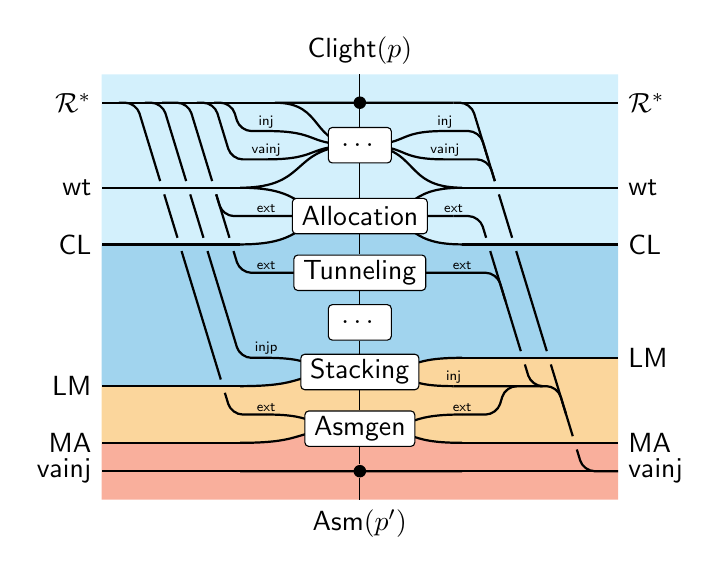
\begin{tikzpicture}[yscale=0.36,thick]
    \tikzset{to path={
      .. controls ($(\tikztostart)!\stens!(\tikztostart -| \tikztotarget)$)
              and ($(\tikztotarget)!\stens!(\tikztotarget -| \tikztostart)$) ..
      (\tikztotarget) \tikztonodes}}

    % Refinement of the incoming convention
    \begin{scope}[xshift=1.3cm,xscale=0.11]
      \draw (-1,14) coordinate (XI1) -- (18,14) node[right] {$\mathcal{R}^*$};
      \draw (0,11) coordinate (AI1) -- (18,11) node[right] {$\kw{wt}$};
      \draw (0, 9) coordinate (AI3) -- (18, 9) coordinate (CLI) node[right] {$\cc{C}{L}$};
      \draw (0, 5) coordinate (SI1) -- (18, 5) coordinate (LMI) node[right] {$\cc{L}{M}$};
      \draw (0, 2) coordinate (GI2) -- (18, 2) coordinate (MAI) node[right] {$\cc{M}{A}$};
      \draw (0, 1) coordinate (RaI) -- (18, 1) node[right] {$\kw{vainj}$};

      % From now on we will use nodes as gaps around crossings
      \tikzset{rounded corners,every node/.style={inner sep=2pt}};

      % The vainj across
      \node (C1) at (4,11) {};
      \node (C2) at (6, 9) {};
      \node (C3) at (10,5) {};
      \node (C4) at (13,2) {};
      \draw (XI1) -- (1,14) -- (C1) -- (C2) -- (C3) -- (C4) -- (14,1) -- (18,1);

      % Spikes off of vainj
      \draw (-2,13) coordinate (XI2) -- (2,13) -- (3,12); % inj
      \draw (-2,12) coordinate (XI3) -- (3,12) -- (C1); % vainj
      \draw (-1, 4) coordinate (SI2) -- (11,4) -- (12,3); % inj

      % Spikes off of that last inj
      \node (C5) at (3,9) {};
      \node (C6) at (7,5) {};
      \draw (-1,10) coordinate (AI2) -- (2,10) -- (C5) -- (C6) -- (8,4) -- (9,4); % ext
      \draw (0, 8) coordinate (TI) -- (4,8) -- (5,7); % ext
      \draw (0, 3) coordinate (GI1) -- (4,3) -- (5,4) -- (6,4); % ext
    \end{scope}

    % Refinement of the outgoing convention
    \begin{scope}[xshift=-1.52cm,xscale=-0.11]
      \draw (-4,14) coordinate (XO1) -- (16,14) node[left] {$\mathcal{R}^*$};
      \draw (0,11) coordinate (AO1) -- (16,11) node[left] {$\kw{wt}$};
      \draw (0, 9) coordinate (AO3) -- (16, 9) coordinate (CLO) node[left] {$\cc{C}{L}$};
      \draw (0, 4) coordinate (SO1) -- (16, 4) coordinate (LMO) node[left] {$\cc{L}{M}$};
      \draw (0, 2) coordinate (GO2) -- (16, 2) coordinate (MAO) node[left] {$\cc{M}{A}$};
      \draw (0, 1) coordinate (RaO) -- (16, 1) node[left] {$\kw{vainj}$};

      % From now on we will use nodes as gaps around crossings
      \tikzset{rounded corners,every node/.style={inner sep=2pt}};

      % Asmgen
      \node (D1) at ( 2, 4) {};
      \node (D2) at ( 7, 9) {};
      \node (D3) at ( 9,11) {};
      \draw (-3, 3) coordinate (GO1) -- (1, 3) -- (D1) -- (D2) -- (D3) -- (12,14) -- (14,14);

      % Stacking
      \node (D5) at ( 4, 9) {};
      \node (D6) at ( 6,11) {};
      \draw (-3, 5) coordinate (SO2) -- (0, 5) -- (D5) -- (D6) -- (9,14) -- (11,14);

      % Tunneling
      \node (D7) at ( 1, 9) {};
      \node (D8) at ( 3,11) {};
      \draw (-3, 8) coordinate (TO)  -- (0, 8) -- (D7) -- (D8);

      % Allocation
      \draw (-3,10) coordinate (AO2) -- (2,10) -- (D8) -- ( 6,14) -- ( 9,14);

      % Frontend
      \draw (-3,12) coordinate (XO3) -- (1,12) -- ( 3,14) -- ( 5,14);
      \draw (-3,13) coordinate (XO2) -- (0,13) -- ( 1,14) -- ( 3,14);
    \end{scope}

    % Nodes
    \begin{scope}
      \begin{pgfonlayer}{nodes}
        \begin{scope}[every node/.style={draw,fill=white,rounded corners=0.5mm,minimum height=0.45cm,inner ysep=0pt}]
          \node[minimum width=0.8cm] (X) at (0,12.5) {\ldots};
          \node (A) at (0,10) {$\kw{Allocation}$};
          \node (T) at (0,8) {$\kw{Tunneling}$};
          \node[minimum width=0.8cm] (C) at (0,6.25) {\ldots};
          \node (S) at (0,4.5) {$\kw{Stacking}$};
          \node (G) at (0,2.5) {$\kw{Asmgen}$};
        \end{scope}
        \begin{scope}[every node/.style={fill=black,circle,inner sep=1.6pt}]
          \node (RC) at (0,14) {};
          \node (RA) at (0,1) {};
        \end{scope}
      \end{pgfonlayer}
    \end{scope}

    \draw[thin]
      (0,15) coordinate (SP) node[above] {$\kw{Clight}(p)$} --
      (X) -- (A) -- (T) -- (C) -- (S) -- (G) -- (RA) --
      (0,0) coordinate (TP) node[below] {$\kw{Asm}(p')$};

    \draw
      (XI1) to (RC.center) to (XO1)
               (X.center) to (XO1)
      (XI2) to (X.center) to (XO2)
      (XI3) to (X.center) to (XO3)
      (AI1) to (X.center) to (AO1)
      (AI1) to (A.center) to (AO1)
      (AI2) to (A.center) to (AO2)
      (AI3) to (A.center) to (AO3)
      (TI)  to (T.center) to (TO)
      (SI1) to (S.center) to (SO1)
      (SI2) to (S.center) to (SO2)
      (GI1) to (G.center) to (GO1)
      (GI2) to (G.center) to (GO2)
      (RaI) to (RA.center) to (RaO);

    % Extra simulation convention labels
    \tiny
    \path[every node/.style={inner sep=0.8pt}]
      (XI2) node[above] {$\kw{inj}$}
      (XI3) node[above] {$\kw{vainj}$}
      (GI1) node[above] {$\kw{ext}$}
      (SI2) node[above] {$\kw{inj}$}
      (TI)  node[above] {$\kw{ext}$}
      (AI2) node[above] {$\kw{ext}$}
      (XO2) node[above] {$\kw{inj}$}
      (XO3) node[above] {$\kw{vainj}$}
      (AO2) node[above] {$\kw{ext}$}
      (TO) node[above] {$\kw{ext}$}
      (SO2) node[above] {$\kw{injp}$}
      (GO1) node[above] {$\kw{ext}$};

    % Region coloring
    \begin{pgfonlayer}{tint}
      \fill[ACMLightBlue\filltint]
        (AI3) to (A.center) to (AO3) --
        (CLO) |- (SP) -| (CLI) -- cycle;
      \fill[ACMBlue\filltint]
        (CLI) -- (AI3) to (A.center) to (AO3) -- (CLO) --
        (LMO) -- (SO1) to (S.center) to (SI1) -- (LMI) -- cycle;
      \fill[ACMOrange\filltint]
        (LMO) -- (SO1) to (S.center) to (SI1) -- (LMI) --
        (MAI) -- (GI2) to (G.center) to (GO2) -- (MAO) -- cycle;
      \fill[ACMRed\filltint]
        (MAI) -- (GI2) to (G.center) to (GO2) -- (MAO) |- (TP) -| cycle;
    \end{pgfonlayer}

  \end{tikzpicture}

\end{frame}

\begin{frame}{Advanced usage: towards heterogeneous verification}
  \centering
  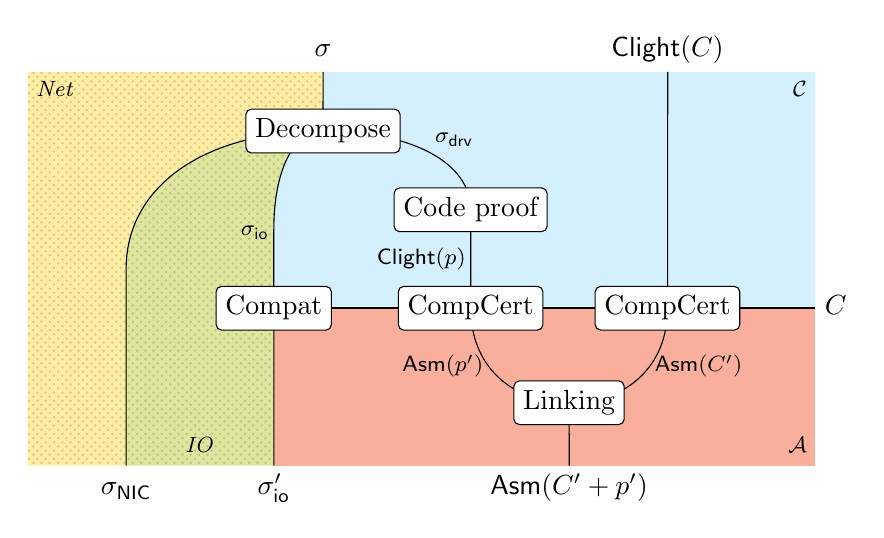
\begin{tikzpicture}[xscale=2.5,yscale=1]
    \tikzset{text height=0.7em,text depth=0.5ex}
    \tikzset{to path={
      .. controls ($(\tikztostart)!\stens!(\tikztostart -| \tikztotarget)$)
              and ($(\tikztotarget)!\stens!(\tikztostart -| \tikztotarget)$) ..
      (\tikztotarget) \tikztonodes}}

    \begin{pgfonlayer}{nodes}
      \begin{scope}[every node/.style={draw,fill=white,rounded corners=2pt}]
        \path
          (0.25,1.5) coordinate (NIC1)
          (1,2) coordinate (IO1)
          (1.25,3.25) coordinate (Def) node {Decompose}
          (1,1) coordinate (IO) node {Compat}
          (2,2.25) coordinate (CP) node {Code proof}
          (2,1) coordinate (T1) node {CompCert}
          (3,1) coordinate (T2) node {CompCert}
          (2.5,-0.2) coordinate (LK) node {Linking};
      \end{scope}
    \end{pgfonlayer}

    % Boundary
    \begin{scope}
      % Corners
      \path (-0.25, 4)       coordinate (ULC)
            ( 2,   -1)       coordinate (LRC)
            ($(ULC -| LRC)$) coordinate (URC)
            ($(ULC |- LRC)$) coordinate (LLC);

      % Source transition systems
      \path ($(Def |- ULC)$) coordinate (Spec) node[above] {$\sigma$};
      \path ($(T2 |- ULC)$) coordinate (CC) node[above] {$\kw{Clight}(C)$};

      % Target transition systems
      \path ($(NIC1 |- LRC)$) coordinate (NIC2) node[below] {$\sigma_\kw{NIC}$};
      \path ($(IO1 |- LRC)$) coordinate (IO2) node[below] {$\sigma_\kw{io}'$};
      \path ($(LK |- LRC)$) coordinate (CD2) node[below] {$\kw{Asm}(C' + p')$};

      % Simulation convention
      \path (3.75,1) coordinate (C) node[right] {$\mathbb{C}$};
    \end{scope}

    % Transition systems
    \begin{scope}[inner sep=1.6pt]
      \footnotesize
      \draw (Def) to (NIC1) -- (NIC2);
      \draw (Def) to node[above right] {$\sigma_\kw{drv}$} (CP.center)
        (CP) -- node[left] {$\kw{Clight}(p)$} (T1)
        (LK.center) to node[left,pos=0.6] {$\kw{Asm}(p')$} (T1.center)
        (LK) -- (CD2);
      \draw (CC) -- (T2)
        (LK.center) to node[right,pos=0.6] {$\kw{Asm}(C')$} (T2.center);
      \draw (Spec)
        -- (Def) to (IO1) node[left] {$\sigma_\kw{io}$}
        -- (IO)
        -- (IO2);
    \end{scope}

    % Simulation convention
    \draw[thick] (IO) -- (C);

    % Colors
    \begin{pgfonlayer}{tint}
      \begin{scope}[every node/.style={black}]
        \footnotesize
        \fill[ACMYellow\filltint] (ULC) -- (Spec) -- (Def)
          to (NIC2) -| (ULC);
        \fill[ACMGreen\filltint]
          (Def) to (NIC1) |- (IO2)
          (Def) to (IO1) -- (IO2);
        \fill[pattern=crosshatch dots,opacity=.15]
          (ULC) -- (Spec) -- (Def) to (IO1) -- (IO2) -| cycle;
        \fill[ACMLightBlue\filltint]
          (Spec) -- (Def) to (IO1) -- (IO) -- (C) |- cycle;
        \fill[ACMRed\filltint] (IO2) rectangle (C);
        \node[below right] at (ULC) {$\li{Net}$};
        \node[above] at ($(NIC2)!0.5!(IO2)$) {$\li{IO}$};
        \node[below left] at ($(CC -| C)$) {$\mathcal{C}$};
        \node[above left] at ($(CD2 -| C)$) {$\mathcal{A}$};
      \end{scope}
    \end{pgfonlayer}
  \end{tikzpicture}
\end{frame}

%}}}

\section*{Conclusion} %{{{

\begin{frame}{Conclusion}
%  Takeaway on CompCertO:
%  careful and compositional treatment of calling conventions
%  make the problem tractable.
%
%  Lesson:
%  scaling up verification will require:
%  \begin{itemize}
%    \item A good formal approach to compositional reasoning,
%      which brings out the common structures in seemingly
%      very different kinds of systems.
%    \item Consolidating progress on compositional semantics
%    \item Get serious about abstraction
%  \end{itemize}
  Vision:
  \begin{center}
    Standardized certified components
    to be assembled into \\
    \textbf{large-scale, heterogeneous certified systems}.
  \end{center}
\end{frame}

%}}}

\fi

\end{document}
